%%%%%%%%%%%%%%%%%%%%%%%%%%%%%%% beamer %%%%%%%%%%%%%%%%%%%%%%%%%%%%%%%%%%%%%%%%%%%%%%%%%
% To run - pdflatex filename.tex
%      acroread filename.pdf
%%%%%%%%%%%%%%%%%%%%%%%%%%%%%%%%%%%%%%%%%%%%%%%%%%%%%%%%%%%%%%%%%%%%%%%%%%%%%%%%%%%%%%%%

\documentclass[compress,oilve,t]{beamer}
\mode<presentation>
\setbeamertemplate{itemize/enumerate body begin}{\normalsize}
\setbeamertemplate{itemize/enumerate subbody begin}{\small}

\usetheme[]{CambridgeUS}
% other themes: AnnArbor, Antibes, Bergen, Berkeley, Berlin, Boadilla, boxes, CambridgeUS, Copenhagen, Darmstadt, default, Dresden, Frankfurt, Goettingen,
% Hannover, Ilmenau, JuanLesPins, Luebeck, Madrid, Maloe, Marburg, Montpellier, PaloAlto, Pittsburg, Rochester, Singapore, Szeged, classic

\usecolortheme{lily}
% color themes: albatross, beaver, beetle, crane, default, dolphin,  fly, lily, orchid, rose, seagull, seahorse, sidebartab, whale, wolverine

\usefonttheme{default}
% font themes: default, professionalfonts, serif, structurebold, structureitalicserif, structuresmallcapsserif


\hypersetup{pdfpagemode=FullScreen} % makes your presentation go automatically to full screen

% define your own colors:
\definecolor{Red}{rgb}{1,0,0}
\definecolor{Blue}{rgb}{0,0,1}
\definecolor{Green}{rgb}{0,1,0}
\definecolor{magenta}{rgb}{1,0,.6}
\definecolor{lightblue}{rgb}{0,.5,1}
\definecolor{lightpurple}{rgb}{0.8, 0.6, 0.9}
\definecolor{gold}{rgb}{.6,.5,0}
\definecolor{orange}{rgb}{1,0.4,0}
\definecolor{hotpink}{rgb}{1,0,0.5}
\definecolor{newcolor2}{rgb}{.5,.3,.5}
\definecolor{newcolor}{rgb}{0,.3,1}
\definecolor{newcolor3}{rgb}{1,0,.35}
\definecolor{darkgreen1}{rgb}{0, .35, 0}
\definecolor{darkgreen}{rgb}{0, .6, 0}
\definecolor{darkred}{rgb}{.75,0,0}
\definecolor{skyblue}{HTML}{75bbfd}

\definecolor{olive}{cmyk}{0.64,0,0.95,0.4}
\definecolor{purpleish}{cmyk}{0.75,0.75,0,0}

% can also choose different themes for the "inside" and "outside"

% \usepackage{beamerinnertheme_______}
% inner themes include circles, default, inmargin, rectangles, rounded

% \usepackage{beamerouterthemesmoothbars}
% outer themes include default, infolines, miniframes, shadow, sidebar, smoothbars, smoothtree, split, tree


\useoutertheme[subsection=true, height=40pt]{smoothbars}

% to have the same footer on all slides
%\setbeamertemplate{footline}[text line]{STUFF HERE!}
\setbeamertemplate{footline}[text line]{} % makes the footer EMPTY
% include packages
%

%show the page numbers in footnote
%\addtobeamertemplate{navigation symbols}{}{%
	%	\usebeamerfont{footline}%
	%	\usebeamercolor[fg]{footline}%
	%	\hspace{1em}%
	%	\insertframenumber/\inserttotalframenumber
	%}

\setbeamercolor{footline}{fg=purpleish}
\setbeamerfont{footline}{series=\bfseries}

%add color to curent subsection
\setbeamertemplate{section in head/foot}{\hfill\tikz\node[rectangle, fill=darkred, rounded corners=1pt,inner sep=1pt,] {\textcolor{white}{\insertsectionhead}};}
\setbeamertemplate{section in head/foot shaded}{\textcolor{darkred}{\hfill\insertsectionhead}}

% Remove bullet of subsections
\setbeamertemplate{headline}
{%
	\begin{beamercolorbox}{section in head/foot}
		\insertsectionnavigationhorizontal{\textwidth}{}{}
	\end{beamercolorbox}%
}


% modify headlline, specially headline size
\setbeamertemplate{headline}{%
	\leavevmode%
	\hbox{%
		\begin{beamercolorbox}[wd=\paperwidth,ht=3.5ex,dp=1.125ex]{palette quaternary}%
			\insertsectionnavigationhorizontal{\paperwidth}{}{\hskip0pt plus1filll}
		\end{beamercolorbox}%
	}
}

\setbeamertemplate{footline}{%
	\leavevmode%
	\hbox{\begin{beamercolorbox}[wd=.5\paperwidth,ht=2.5ex,dp=1.125ex,leftskip=.3cm plus1fill,rightskip=.3cm]{author in head/foot}%
			\usebeamerfont{author in head/foot}\insertshortauthor ~ \insertshortinstitute
		\end{beamercolorbox}%
		\begin{beamercolorbox}[wd=.5\paperwidth,ht=2.5ex,dp=1.125ex,leftskip=.3cm,rightskip=.3cm plus1fil]{title in head/foot}%
			\usebeamerfont{title in head/foot}\insertshorttitle\hfill\insertframenumber\,/\,\inserttotalframenumber
	\end{beamercolorbox}}%
	\vskip0pt%
}


%\setbeamertemplate{navigation symbols}{}

%Write \usepackage{etex} just after the \documentclass line (it should be the first loaded package).
\usepackage{etex}
\usepackage{subcaption}
\usepackage{multicol}
\usepackage{amsmath}
\usepackage{epsfig}
\usepackage{graphicx}
\usepackage[all,knot]{xy}
\xyoption{arc}
\usepackage{url}
\usepackage{multimedia}
\usepackage{hyperref}
\hypersetup{colorlinks,linkcolor=blue,citecolor=redorange,urlcolor=darkred}
\usepackage{multirow}
\usepackage[justification=centering,font={scriptsize}]{caption}
\usepackage{pgf}
\usepackage{fontspec}
\usepackage{import}
\usepackage{textpos}
\usepackage{bm}
\usepackage{mathtools}
\usepackage{relsize}
\usepackage[notransparent]{svg}
\usepackage{caption}
\usepackage{hyperref}
\usepackage[font={scriptsize}]{caption}
%\setsansfont[Scale=MatchLowercase, BoldFont = * Bold, ItalicFont = * Italic]{Caladea}

%\usepackage{enumitem,xcolor}
%\newcommand{\labelitemi}{$\blacksquare$}
%\newcommand{\labelitemii}{$\diamond$}
%\newcommand{\labelitemiii}{$\square$}
%\newcommand{\labelitemiv}{$\ast$}
%\setbeamercolor*{item}{fg=red}


\usefonttheme{professionalfonts} 
\setbeamertemplate{itemize item}{\color{skyblue}$\blacksquare$}
\setbeamertemplate{itemize subitem}{\color{hotpink}$\triangleright$}
\setbeamertemplate{itemize subsubitem}{\color{orange}$\bullet$}


\usepackage{anyfontsize}
\usepackage{t1enc}
\usepackage{tikz}
\usepackage{pgfplots}
\usetikzlibrary{calc,trees,positioning,arrows,chains,shapes.geometric,decorations.pathreplacing,decorations.pathmorphing,shapes,matrix,shapes.symbols}


\usepackage{xcolor}
\newcommand{\tc}[2]{
	\textcolor{#1}{\hspace{-2pt}#2\hspace{-2pt}}
}

\newtheorem{proposition}[theorem]{Proposition}
\newtheorem{remark}[theorem]{Remark}
\newtheorem{assumption}[theorem]{Assumption}

%\usepackage{fontspec,unicode-math}
%\setmainfont[Scale=0.9]{Nimbus Roman No9 L}
%\setmonofont[Scale=0.9]{Monaco}
\setsansfont[Scale=1]{Times New Roman}

\newcommand{\vect}[1]{\boldsymbol{#1}}

\definecolor{strings}{rgb}{.624,.251,.259}
\definecolor{keywords}{rgb}{.893,.188,.01}
\definecolor{comment}{rgb}{.322,.451,.322}

%\usepackage{smartdiagram}
%\usesmartdiagramlibrary{additions}
%%%%%%%%%%%%%%%%%%%%%%%%%%%%%%%%%%%%%%%%%%%%%%%%%%%%%%%%%%%%%%%%%%%%%%%%%%%%%%%%%%%%%%%%%%%%
%%%%%%%%%%%%%%%%%%%%%%%%%%%%%% Title Page Info %%%%%%%%%%%%%%%%%%%%%%%%%%%%%%%%%%%%%%%%%%%
%%%%%%%%%%%%%%%%%%%%%%%%%%%%%%%%%%%%%%%%%%%%%%%%%%%%%%%%%%%%%%%%%%%%%%%%%%%%%%%%%%%%%%%%%%
\title{Scientific Computation Project}
\author{Brain Tumor Classification (MRI)}
\institute[]{MSCS Department \newline University of Tehran \newline \newline Mohammad Zamani \newline 610399135}
\date[\today]{}
\titlegraphic{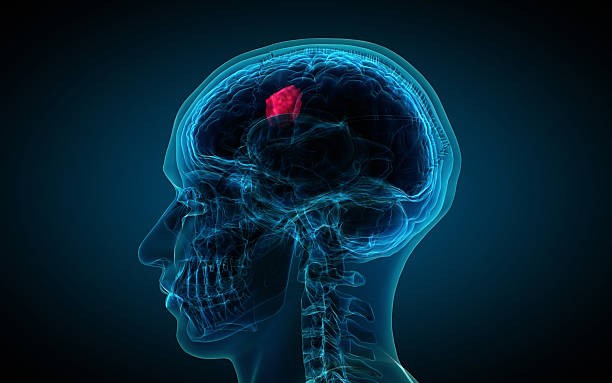
\includegraphics[scale=.3]{Figs/intro.png}}

%%%%%%%%%%%%%%%%%%%%%%%%%%%%%%%%%%%%%%%%%%%%%%%%%%%%%%%%%%%%%%%%%%%%%%%%%%%%%%%%%%%%%%%%%%
%%%%%%%%%%%%%%%%%%%%%%%%%%%%%% Begin Your Document %%%%%%%%%%%%%%%%%%%%%%%%%%%%%%%%%%%%%%%
%%%%%%%%%%%%%%%%%%%%%%%%%%%%%%%%%%%%%%%%%%%%%%%%%%%%%%%%%%%%%%%%%%%%%%%%%%%%%%%%%%%%%%%%%%
\begin{document}
	
%%%%%%%%%%%%%%%%%%%%%%%%%%%%%%%%%%%%%%%%%%%%%%%%%%%%%%%%%%%%%%%%%%%%%%%%%%%%%%%%%%%%%%%%%%
\fontsize{9}{9}
\begin{frame}[noframenumbering, plain]
	\titlepage
\end{frame}

%%%%%%%%%%%%%%%%%%%%%%%%%%%%%%%%%%%%%%%%%%%%%%%%%%%%%%%%%%%%%%%%%%%%%%%%%%%%%%%%%%%%%%%%%%
%\section{Brain Tumor}
%\import{Sections/}{section0.tex}
%\section{SLP}
%\import{Sections/}{section1.tex}
%\section{MLP}
%\import{Sections/}{section2.tex}
%\section{=Gradient Descent}
%\import{Sections/}{section3.tex}
%\section{Training MLPs}
%\import{Sections/}{section4_training.tex}
%%%%%%%%%%%%%%%%%%%%%%%%%%%%%%%%%%%%%%%%%%%%%%%%%%%%%%%%%%%%%%%%%%%%%%%%

%%%%%%%%%%%%%%%%%%%%%%%%%%[Brain Tumor]%%%%%%%%%%%%%%%%%%%%%%%%%%%%%%%%%%%%%%%%%%%%%%%%%%%%%
\section{Brain Tumor}
\begin{frame}{What is Brain Tumor?}
	\begin{itemize}
		\item A brain tumour is a growth of cells in the brain that multiplies in an 						abnormal, uncontrollable way.
	\end{itemize}
	\newline
	\newline
	\newline		
	\begin{figure}[!b]
		\centering
		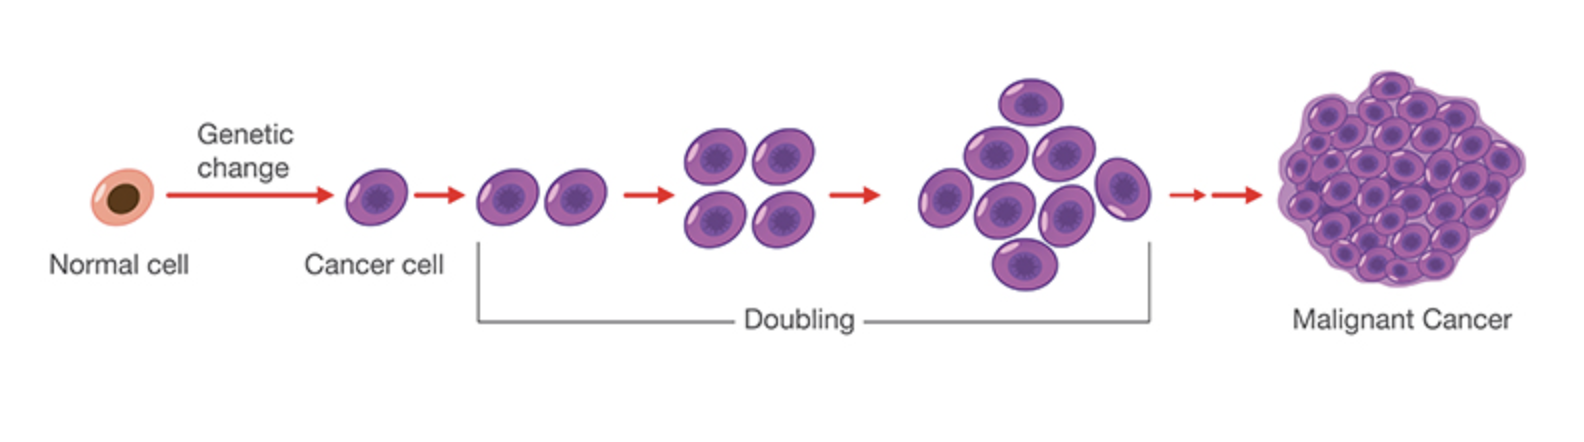
\includegraphics[width=0.9\textwidth]{Figs/cancer-process2}
		\caption{Process of cancer cell development}
	\end{figure}
\end{frame}

\begin{frame}{Brain Tumors}
	\begin{itemize}
		\item[1.] primary brain tumors 
		\item[2.] secondary brain tumors
	\end{itemize}
	\begin{figure}[H]
		\centering
		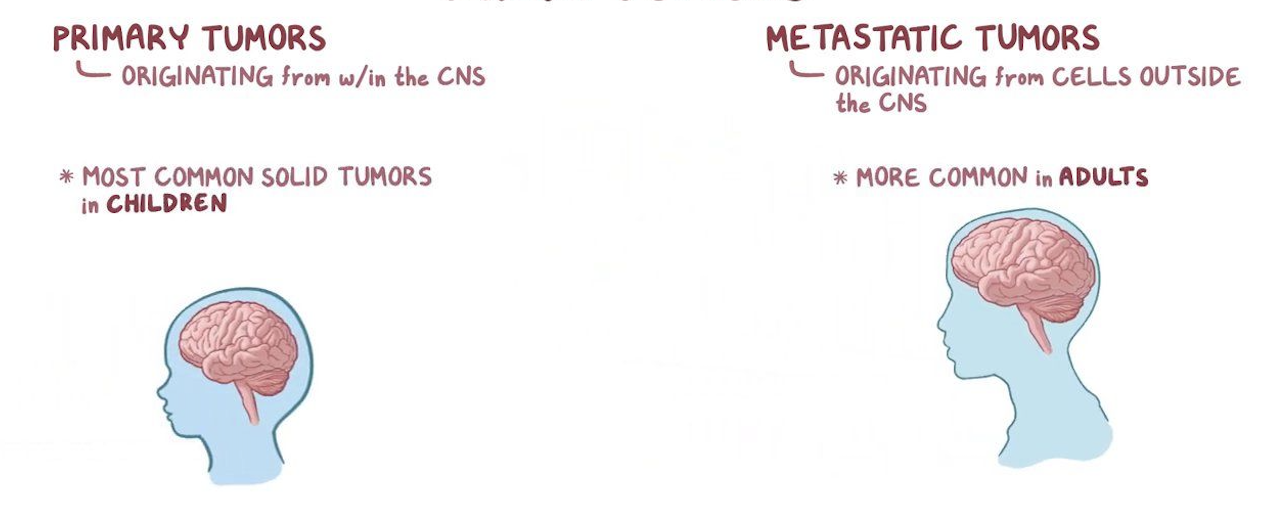
\includegraphics[width=0.9\textwidth]{Figs/BrainTumorTypes}
		\caption{Primary vs Secondary brain tumor}
	\end{figure}
\end{frame}


\begin{frame}{Types}
	\newline
	\begin{itemize}
		\item There are many types of brain tumors. The type of brain tumor is based on the 				kind of cells that make up the tumor.
			\newline
		\begin{itemize}
			\item Glioma 
			\newline
			\item Meningioma
			\newline
			\item Pituitary
			\newline
		\end{itemize}	
	\end{itemize}
\end{frame}

\begin{frame}{Glioma}
	\begin{itemize}
		\item Glioma is a growth of cells that starts in the brain or spinal cord. The cells in a glioma look similar to healthy brain cells called glial cells. Glial cells surround nerve cells and help them function.
		\newline
		\item Gliomas are most common in adults between ages 45 and 65 years old. But glioma can happen at any age. 
	\end{itemize}
	\begin{figure}[H]
		\centering
		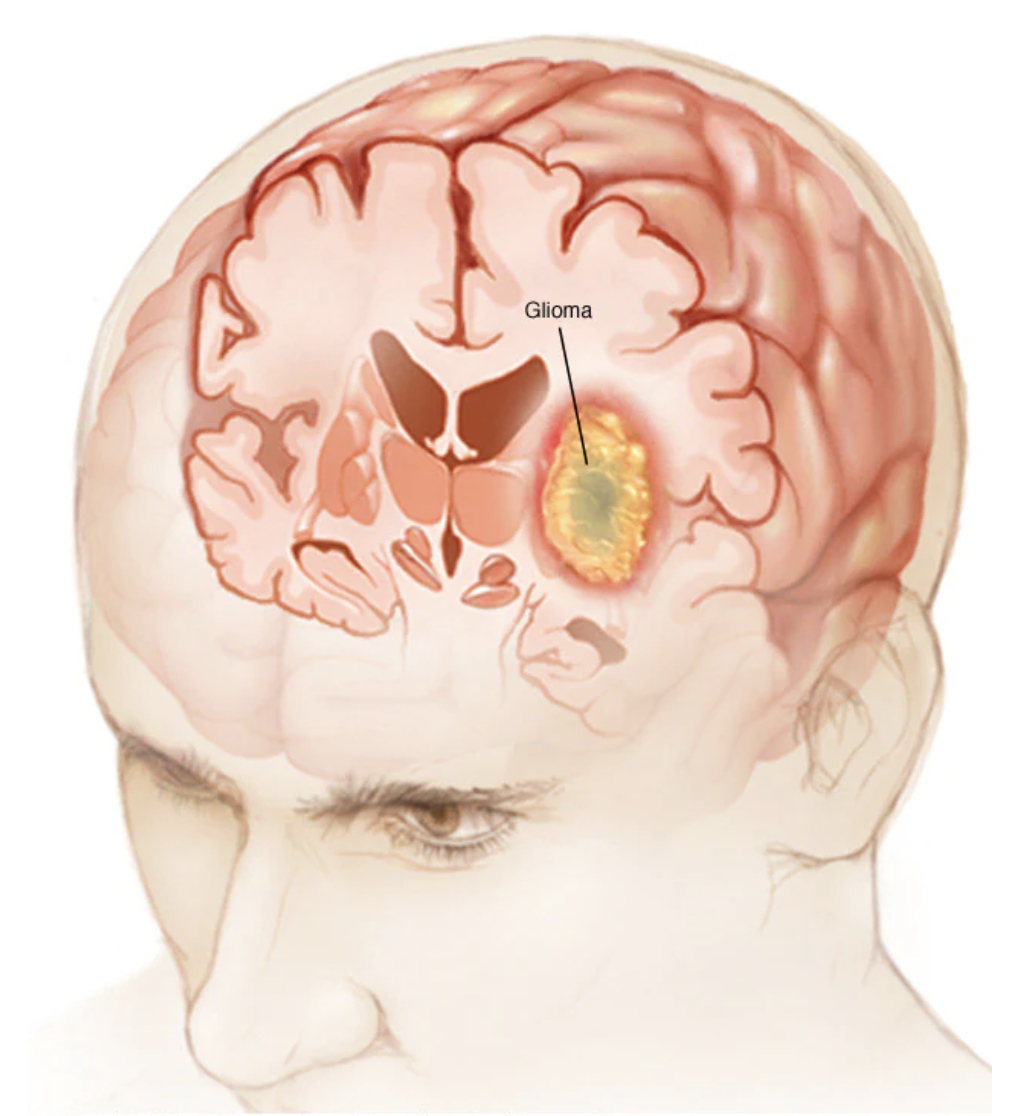
\includegraphics[width=0.3\textwidth]{Figs/glioma}
	\end{figure}
\end{frame}


\begin{frame}{Meningioma}
	\begin{itemize}
		\item A meningioma is a tumor that grows from the membranes that surround the brain and spinal cord, called the meninges. A meningioma is not a brain tumor, but it may press on the nearby brain, nerves and vessels.
		\newline
		\item Meningioma is the most common type of tumor that forms in the head.
	\end{itemize}
	\begin{figure}[H]
		\centering
		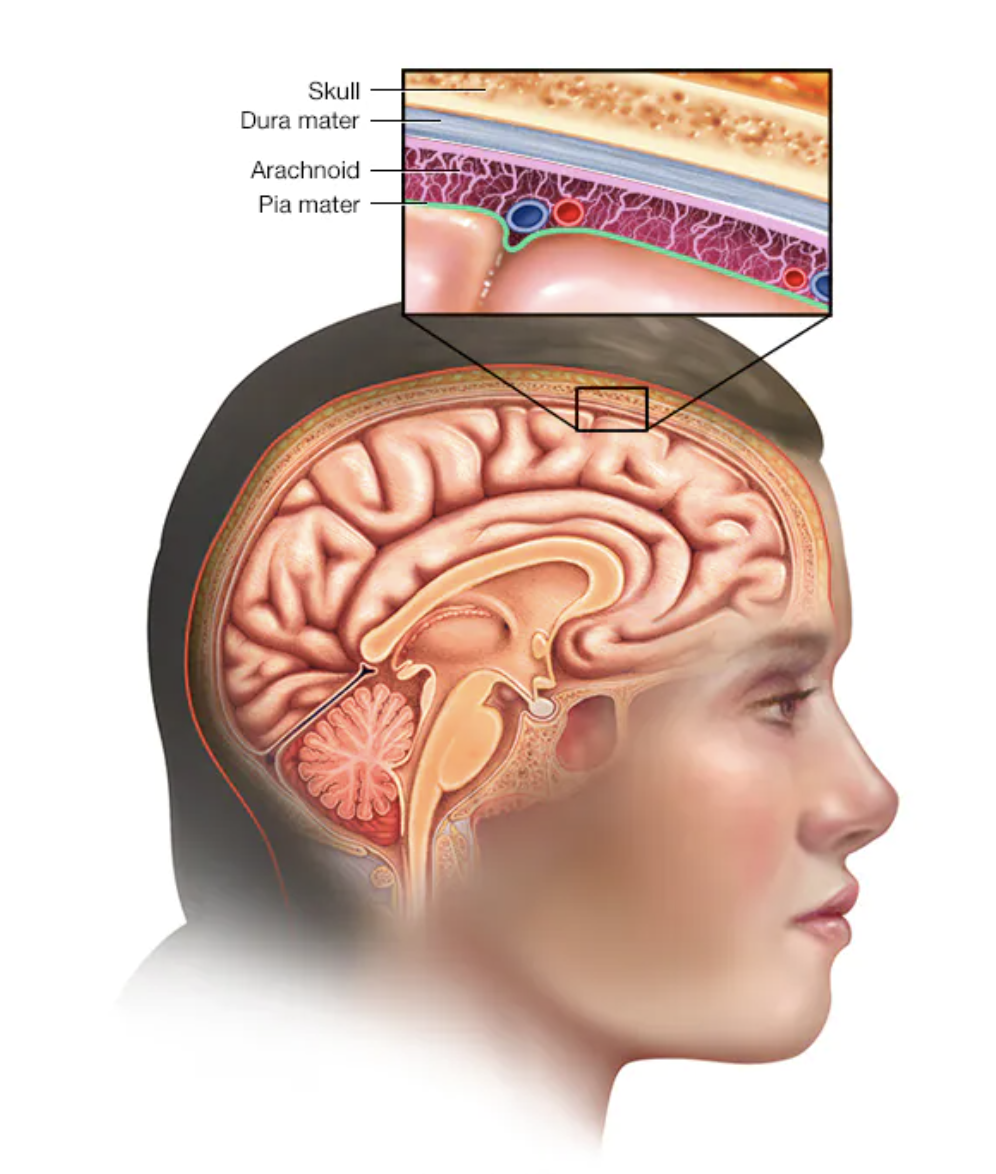
\includegraphics[width=0.3\textwidth]{Figs/meningioma}
	\end{figure}
\end{frame}

\begin{frame}{Pituitary}
	\begin{itemize}
		\item Pituitary tumors are unusual growths that develop in the pituitary gland. This gland is an organ about the size of a pea. It's located behind the nose at the base of the brain. 
		\newline
		\item Most pituitary tumors are benign. That means they are not cancer. 
	\end{itemize}
	\begin{figure}[H]
		\centering
		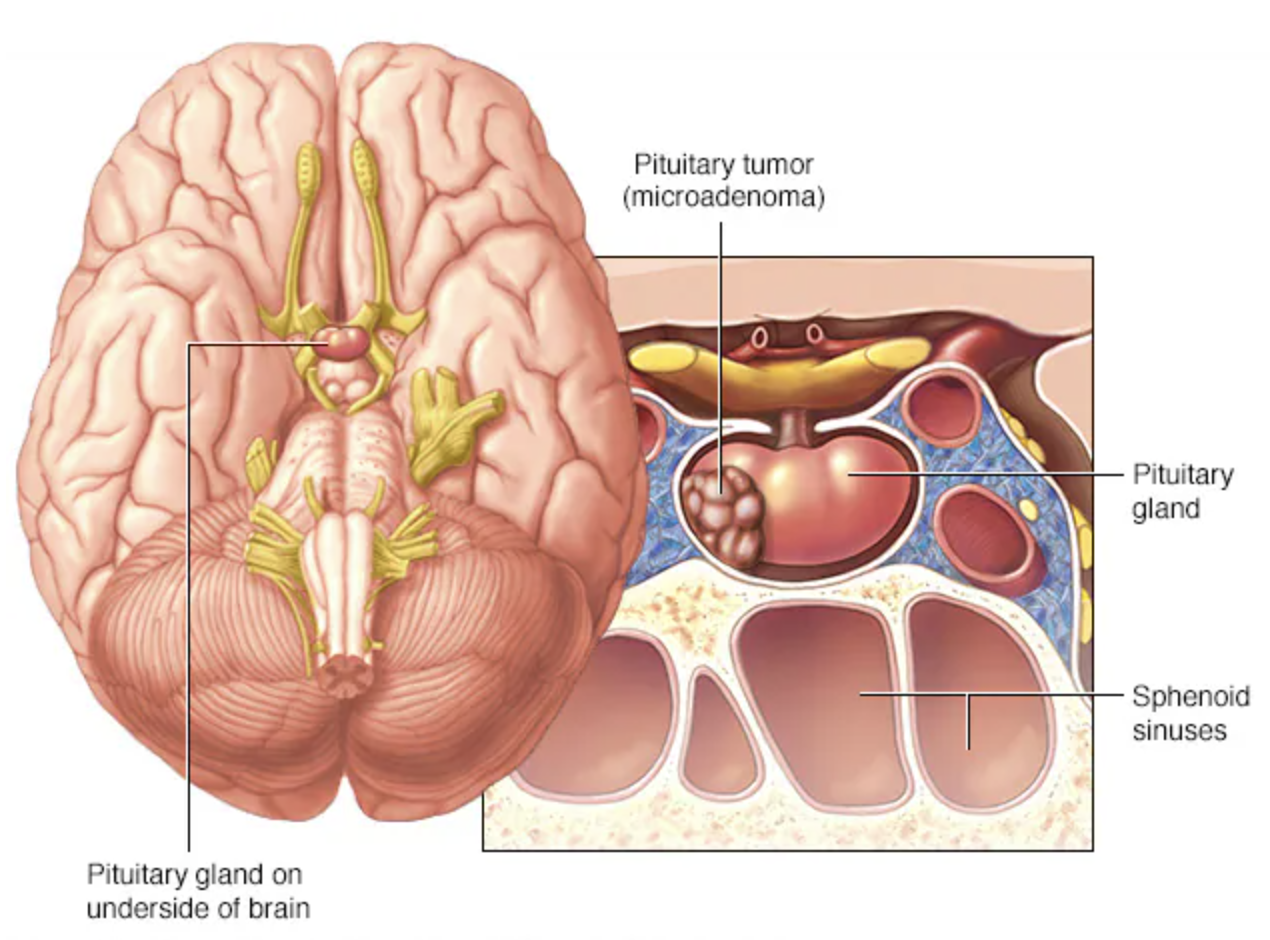
\includegraphics[width=0.5\textwidth]{Figs/pituitary}
	\end{figure}
\end{frame}

%%%%%%%%%%%%%%%%%%%%%%%%%%[MRI]%%%%%%%%%%%%%%%%%%%%%%%%%%%%%%%%%%%%%%%%%%%%%%%%%%%%%%%%%%%%%
\section{MRI}
\begin{frame}{MRI}
\begin{figure}[H]
		\centering
		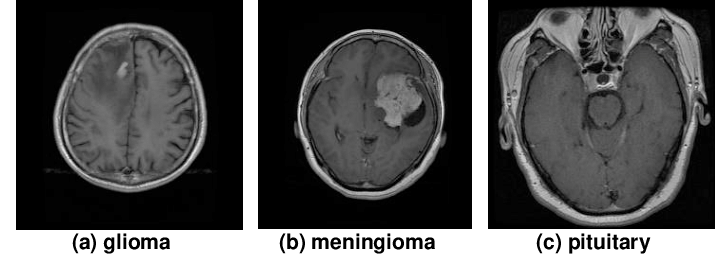
\includegraphics[width=0.9\textwidth]{Figs/The-brain-tumor-dataset-sample-for-three-classes-a-glioma-b-meningioma-c.png}
	\end{figure}
\end{frame}

%%%%%%%%%%%%%%%%%%%%%%%%%%[Single Layer Perceptron]%%%%%%%%%%%%%%%%%%%%%%%%%%%%%%%%%%%%%%%%%%
\section{SLP}
\begin{frame}{Biological Analogy}
	\begin{figure}[H]
		\centering
		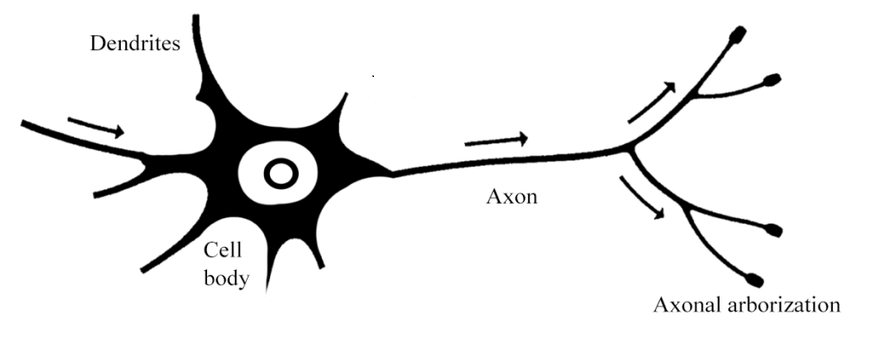
\includegraphics[width=0.9\textwidth]{Figs/biological_neuron.png}
		\caption{Anatomy of a biological neuron \cite{biological-and-nn-neuron}.}
	\end{figure}
\end{frame}

\begin{frame}{Activation Functions}
	\begin{figure}[H]
		\centering
		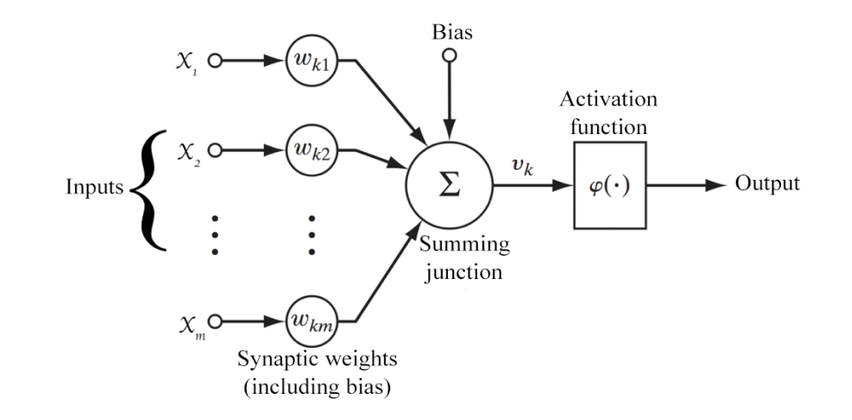
\includegraphics[width=0.9\textwidth]{Figs/nn_neuron.png}
		\caption{Neural network neuron \cite{biological-and-nn-neuron}.}
	\end{figure}
\end{frame}

\begin{frame}{Activation Functions}
	\begin{figure}[H]
		\centering
		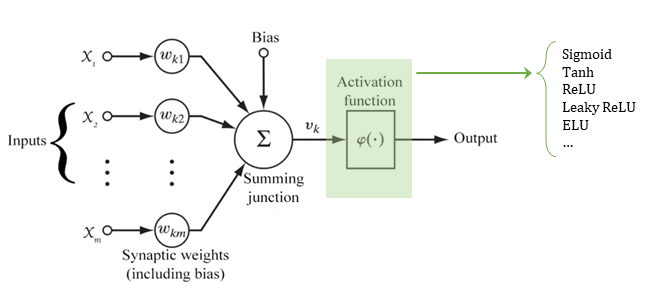
\includegraphics[width=0.9\textwidth]{Figs/activation_function_1.png}
		\caption{Activation function}
	\end{figure}
\end{frame}



\begin{frame}{Activation Functions}
	\begin{figure}[H]
		\centering
		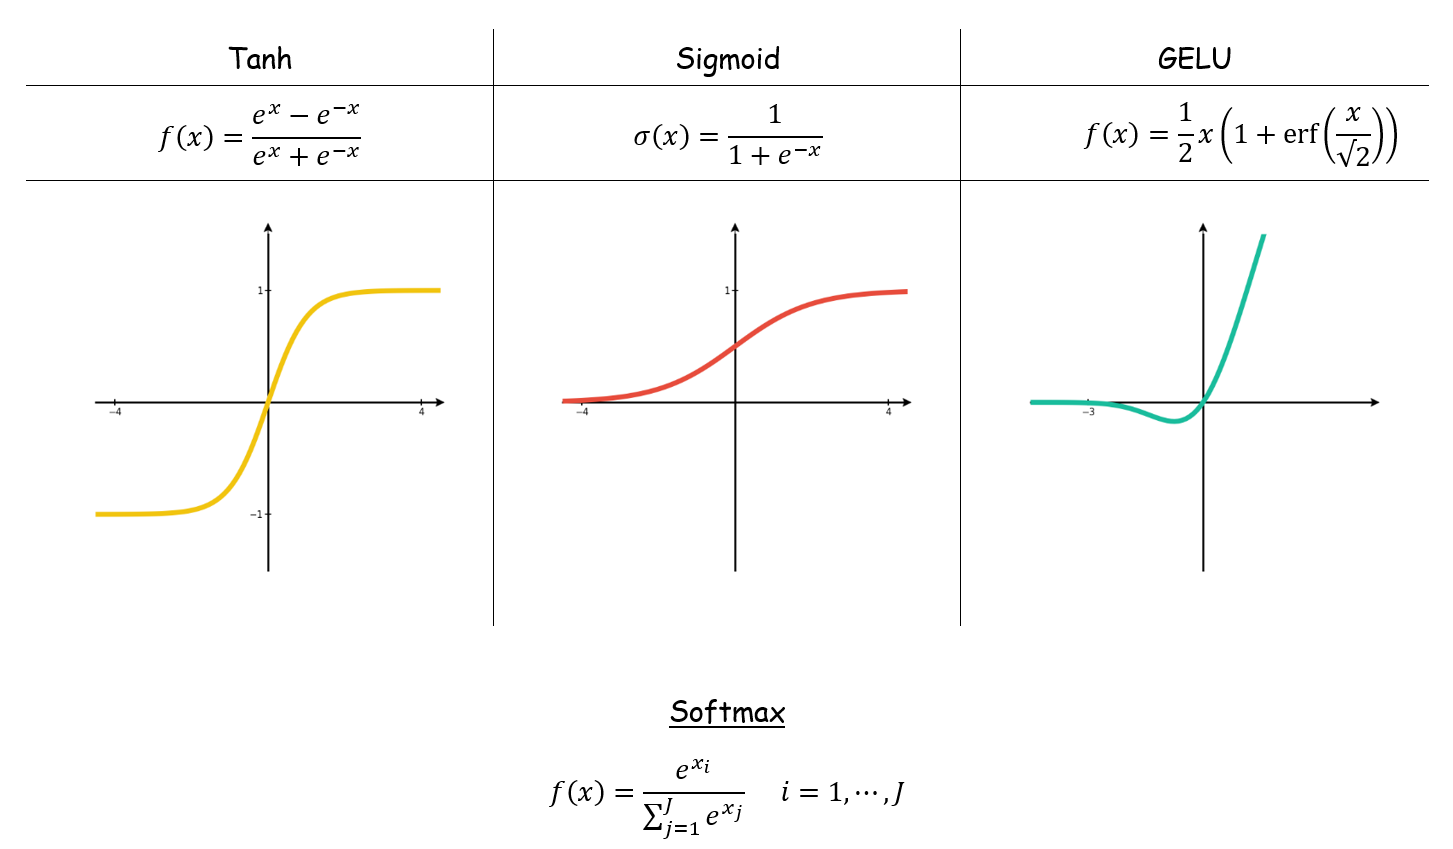
\includegraphics[width=1\textwidth]{Figs/section_1/activation_functions_2.PNG}
	\end{figure}
\end{frame}

\begin{frame}{Gradient Descent}
	\begin{figure}[H]
		\centering
		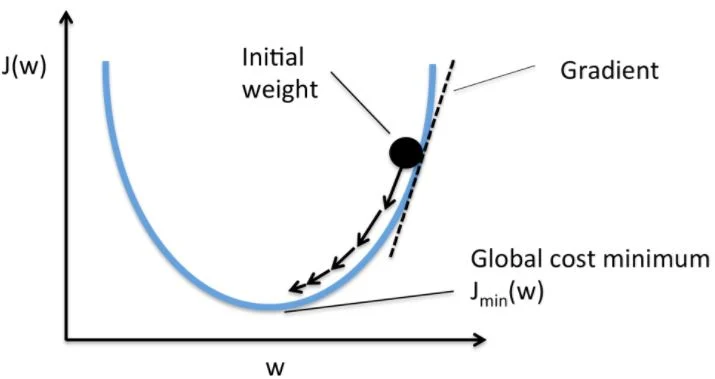
\includegraphics[width=0.70\textwidth]{Figs/gradient_descent2.png}
		\caption{Gradient descent \cite{gradient-descend2}.}
	\end{figure}
\end{frame}

\begin{frame}{Gradient Descent}
	\begin{itemize}
		\item Let's define our problem:
		\begin{itemize}
			\item We have dataset $\mathcal{D} = \{x^{i}, y^{(i)}\}_{i=1}^{n}$.
			\medskip
			\item $f$ is a single layer perceptron.
			\medskip
			\item Define $\hat{y}^{(i)} = f(x^{(i)})$.
		\end{itemize}
		\medskip
		\item We want to minimize following cost function:
		$$
		\mathcal{J}(\bm{w})  = \frac{1}{2} \sum_{i=1}^{n} (y^{(i)} - \hat{y}^{(i)})^2
		$$
		\medskip
		\item We are going to use gradient descent algorithm. $\bm{w}$ will be updated as follows:
		\[
		\bm{w}^{t+1} = \bm{w}^{t} - \eta \nabla_{\bm{w}} \mathcal{J}
		\]
	\end{itemize}
\end{frame}

%%%%%%%%%%%%%%%%%%%%%%%%%%[Multi Layer Perceptron]%%%%%%%%%%%%%%%%%%%%%%%%%%%%%%%%%%%%%%%%%%%
\section{MLP}
\begin{frame}{Limitations of SLP}
	\begin{itemize}
		\item What are the limitations of SLP?
		\item Can we learn all functions with SLP?
	\end{itemize}
	\begin{figure}[H]
		\centering
		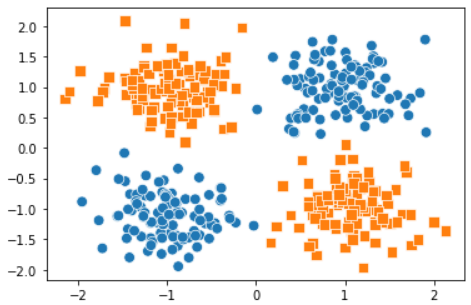
\includegraphics[width=0.6\textwidth]{Figs/xor.png}
		\caption{The XOR function is not linear separable.}
	\end{figure}
\end{frame}

\begin{frame}{Multi-Layer Perceptron}
	\begin{itemize}
		\item So if we know some $f_1, \cdots, f_4$ we can use SLP to solve problem.
	\end{itemize}
	\begin{figure}[H]
		\centering
		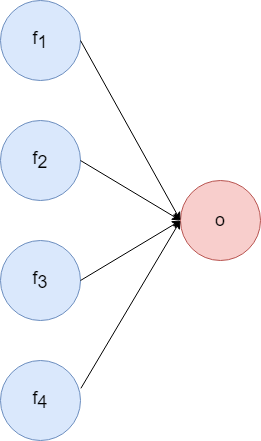
\includegraphics[height=0.45\textheight]{Figs/feature_space.png}
		\caption{Using feature space $f$ to solve problem.}
	\end{figure}
	\begin{itemize}
		\item How to learn this $f_i$s? Use SLP!
	\end{itemize}
\end{frame}

\begin{frame}{Multi-Layer Perceptron}
	\begin{itemize}
		\item We can use inputs ($x_i$) to learn features ($f_i$)
	\end{itemize}
	\begin{figure}[H]
		\centering
		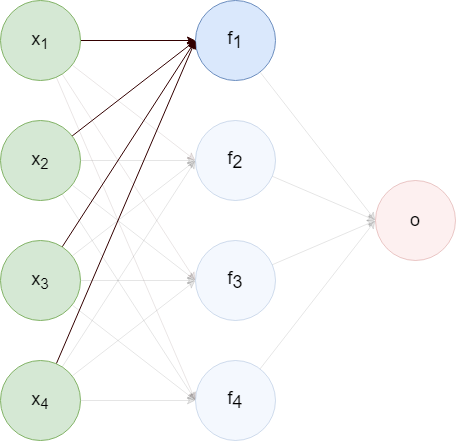
\includegraphics[height=0.45\textheight]{Figs/learn_features.png}
		\caption{Using inputs to learn features.}
	\end{figure}
	\begin{itemize}
		\item What if $f_i$s are not sufficient? We can add more layers!
	\end{itemize}
\end{frame}

\begin{frame}{Multi-Layer Perceptron}
	\begin{itemize}
		\item Adding more layers we will have a bigger network.
	\end{itemize}
	\begin{figure}[H]
		\centering
		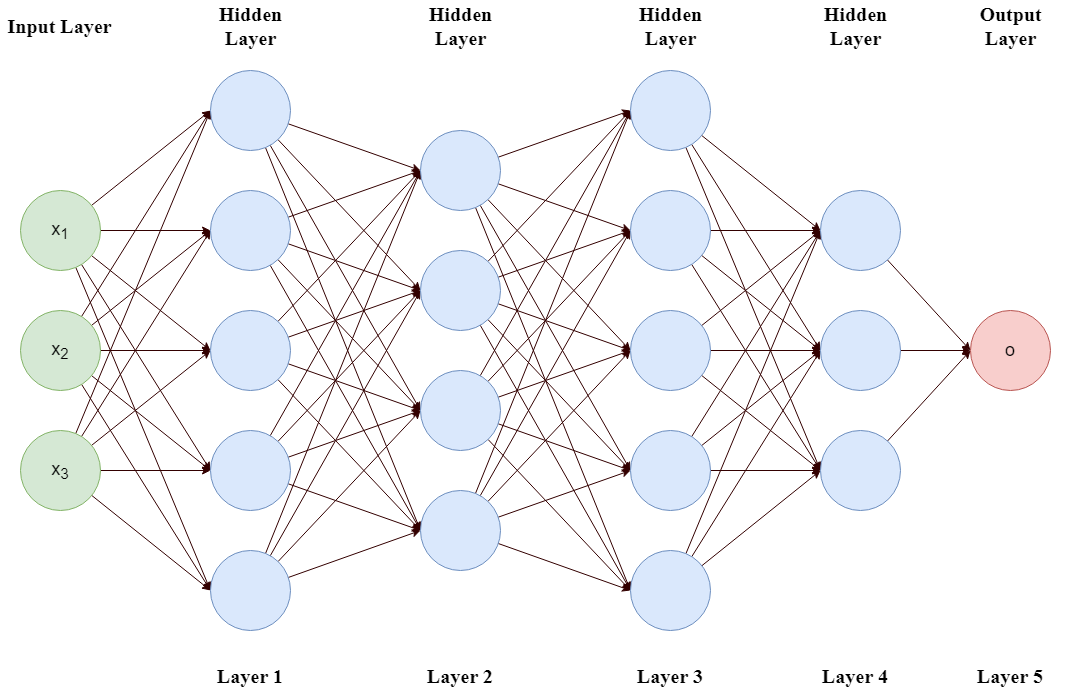
\includegraphics[width=0.8\textwidth]{Figs/5layer_mlp.png}
		\caption{A 5 layer MLP.}
	\end{figure}
\end{frame}


\begin{frame}{Architecture of MLPs}
	\begin{itemize}
		\item Important questions:
		\begin{itemize}
			\item How many hidden layers should we have?
			\item In each hidden layer, how many neurons should we have?
		\end{itemize}
	\end{itemize}
	\begin{figure}[H]
		\centering
		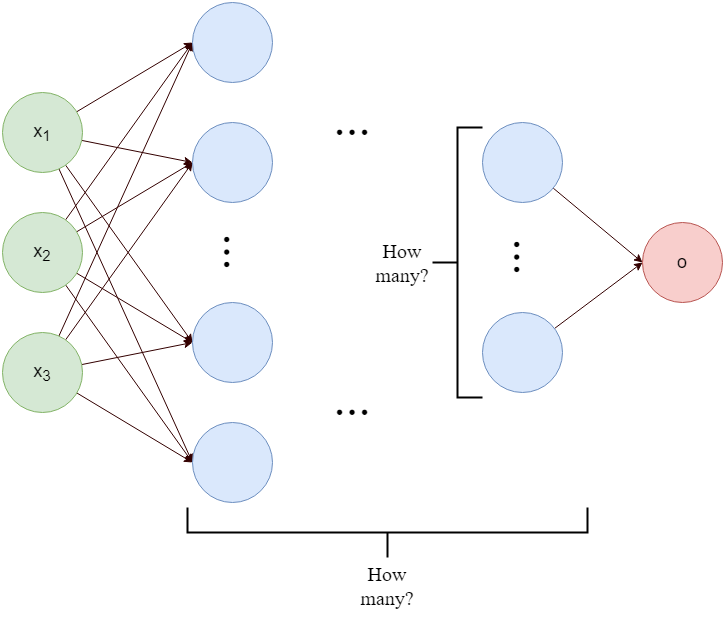
\includegraphics[height=0.6\textheight]{Figs/how_many_layer.png}
		\caption{How many layers and neurons should we have?}
	\end{figure}
\end{frame}


\begin{frame}{Architecture of MLPs}
	\begin{itemize}
		\item In practice:
		\begin{itemize}
			\item You have limited resources
			\item There is no universal rule to choose this hyperparameters
			\item Need to experiment for different number of layers and neurons in each layer
		\end{itemize}
	\end{itemize}
	\begin{figure}[H]
		\centering
		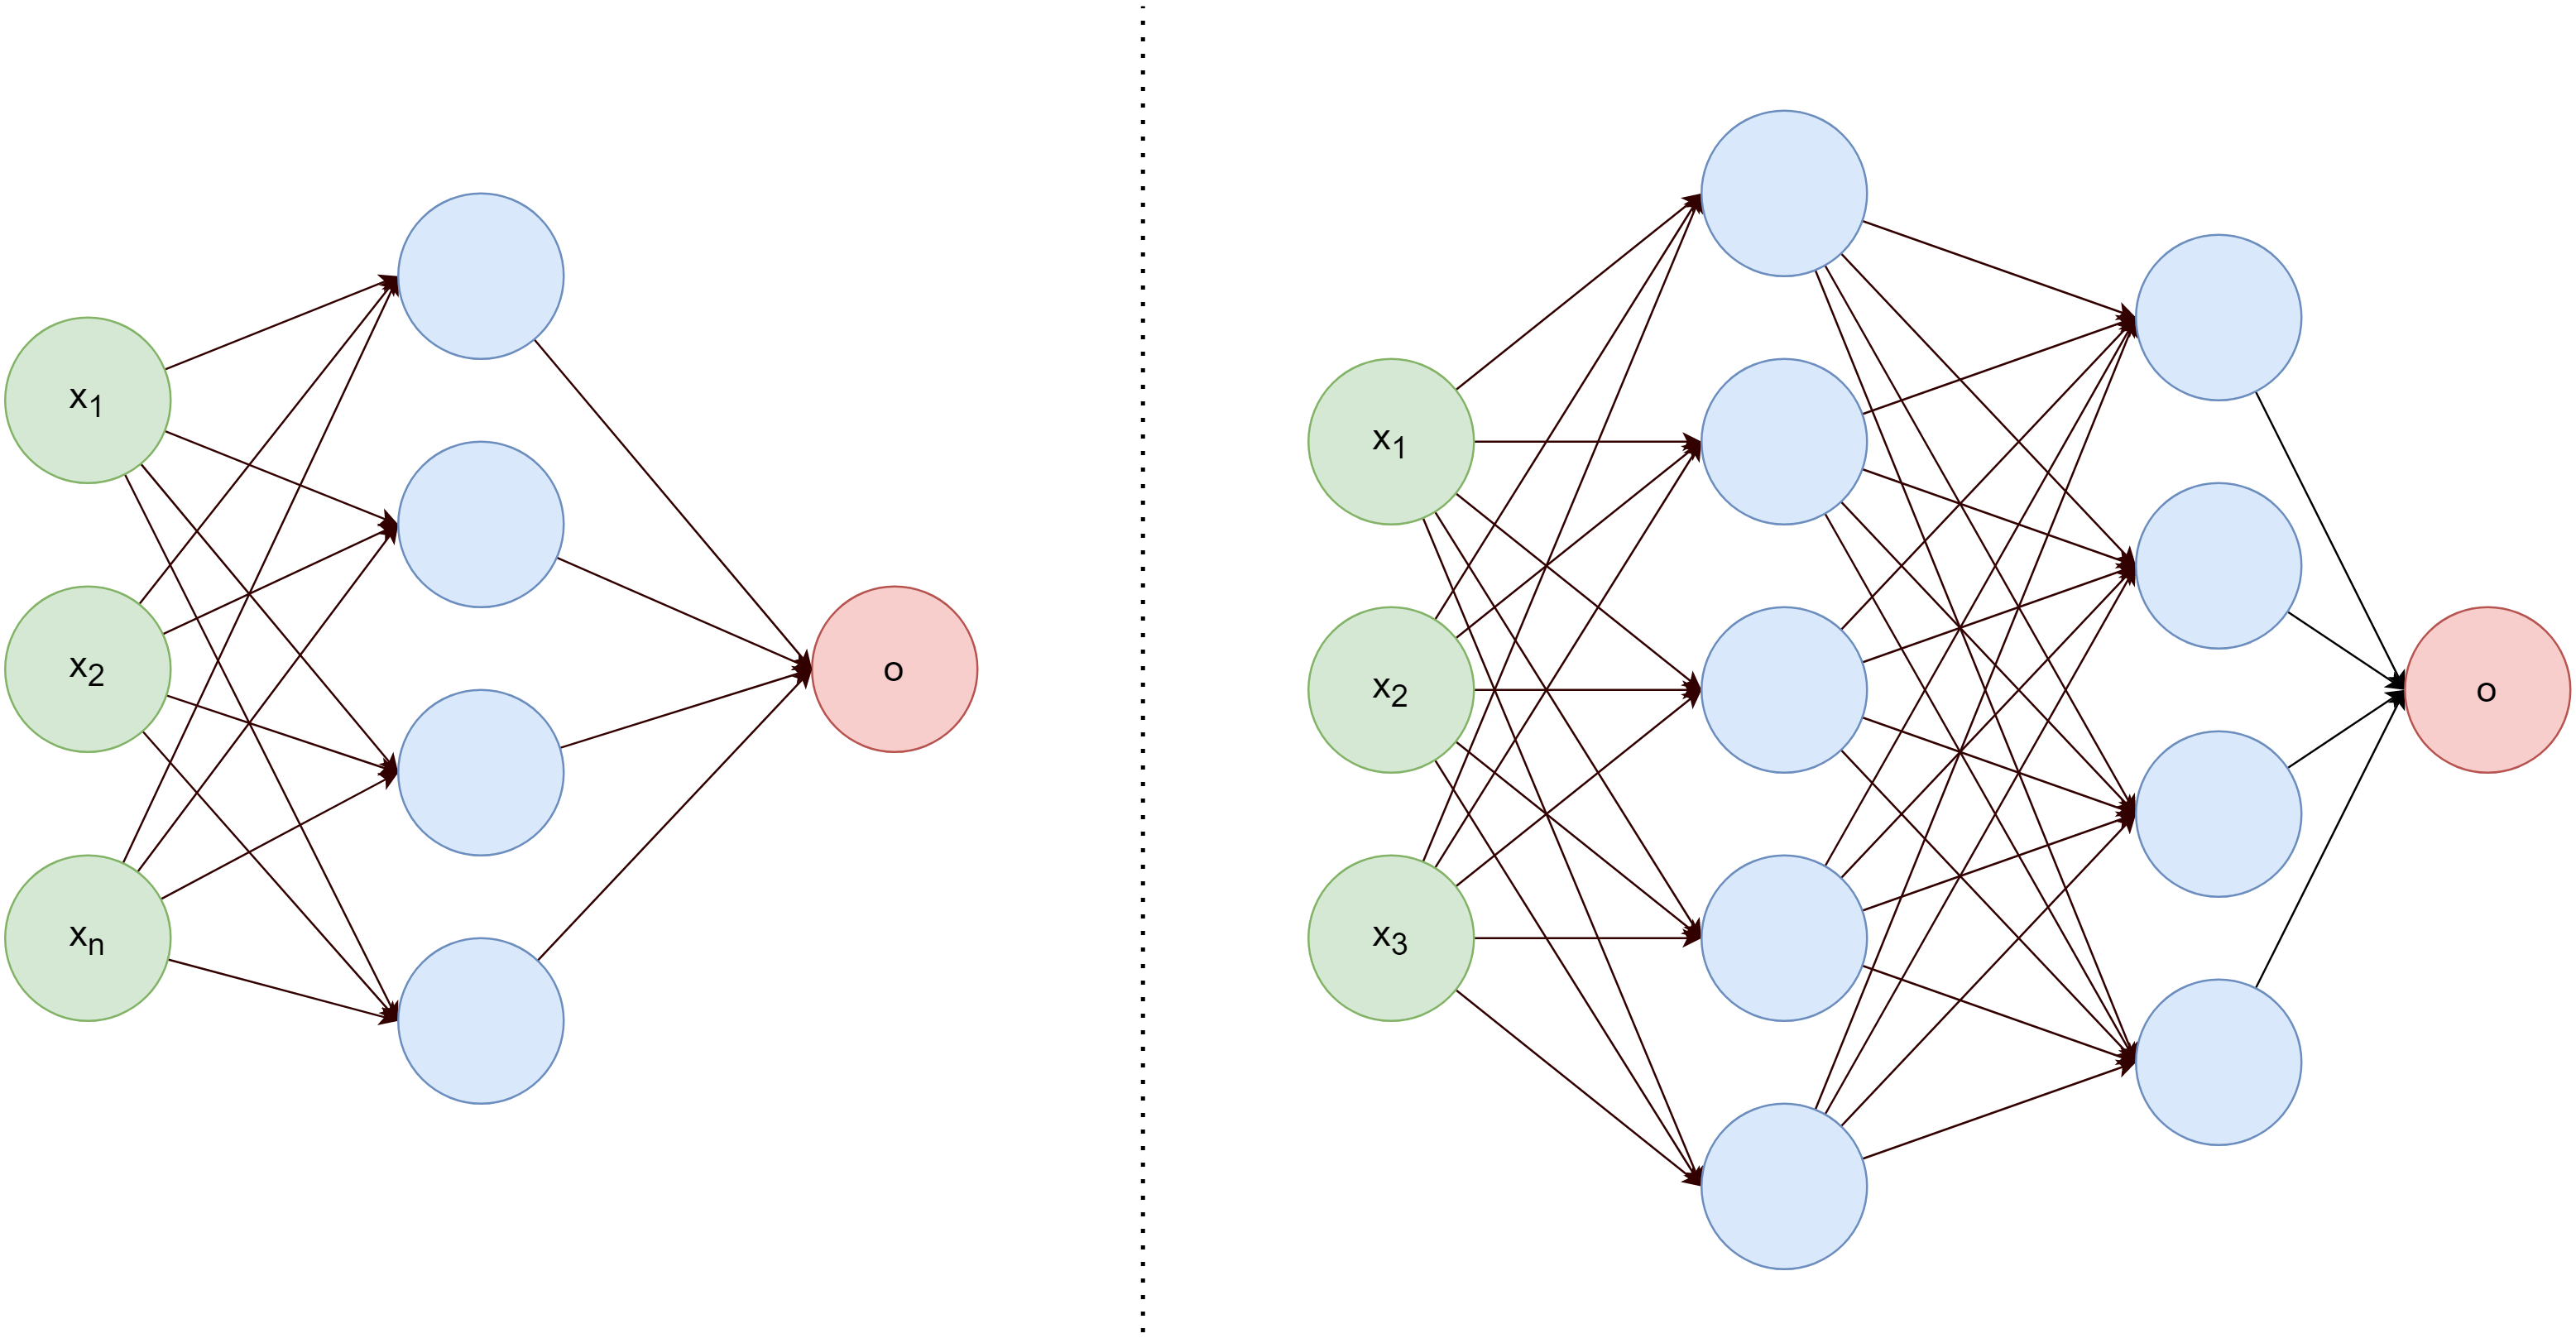
\includegraphics[width=0.6\textwidth]{Figs/experiment_arch.png}
		\caption{Experiment for different architecture and choose the best model.}
	\end{figure}
\end{frame}

\begin{frame}{XOR problem}
	\begin{itemize}
		\item Now let's solve XOR problem with MLPs.
		\item We have two binary inputs, build an MLP to calculate their \textbf{XOR}.
		\medskip
		\medskip
		\item First let's build logical \textbf{AND} and \textbf{OR} functions.
	\end{itemize}
	\begin{figure}[H]
		\centering
		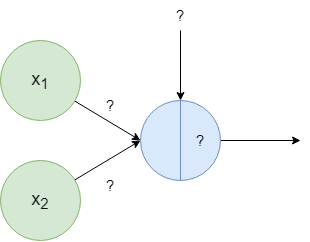
\includegraphics[width=0.35\textwidth]{Figs/solve_and_or_gate.png}
		\caption{We need to find weights, biases and activation function.}
	\end{figure}
\end{frame}

\begin{frame}{XOR problem}
	\begin{figure}
		\centering
		\begin{subfigure}[b]{0.25\textwidth}
			\centering
			$\vcenter{\hbox{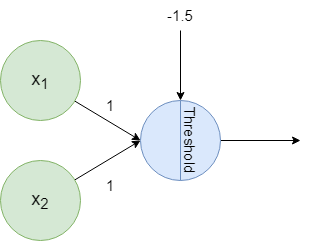
\includegraphics[width=\textwidth]{Figs/and_gate.png}}}$
			\caption{$x_1 \wedge x_2$}
		\end{subfigure}
		\hspace*{0.5em}
		\begin{subfigure}[b]{0.25\textwidth}
			\centering
			$\vcenter{\hbox{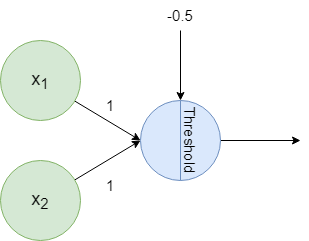
\includegraphics[width=\textwidth]{Figs/or_gate.png}}}$
			\caption{$x_1 \vee x_2$}
		\end{subfigure}
		\hspace*{0.5em}
		\begin{subfigure}[b]{0.25\textwidth}
			\centering
			$\vcenter{\hbox{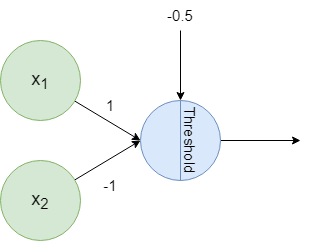
\includegraphics[width=\textwidth]{Figs/and_not_gate.png}}}$
			\caption{$x_1 \wedge \overline{x_2}$}
		\end{subfigure}
	\end{figure}
	\begin{figure}[H]
		\centering
		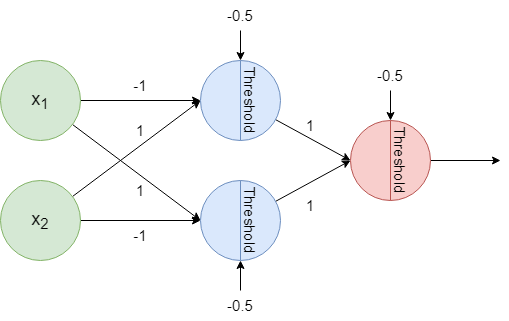
\includegraphics[height=0.35\textheight]{Figs/xor_gate.png}
		\caption{MLP for XOR function.}
	\end{figure}
\end{frame}




\begin{frame}{Learning MLPs}
	\begin{itemize}
		\item Till here we have used networks with predefined weights and biases.
		\item How to learn these parameters?
		\medskip
		\medskip
		\medskip
		\item The idea is to use gradient descent
	\end{itemize}
	\begin{figure}
		\centering
		\begin{subfigure}[b]{0.3\textwidth}
			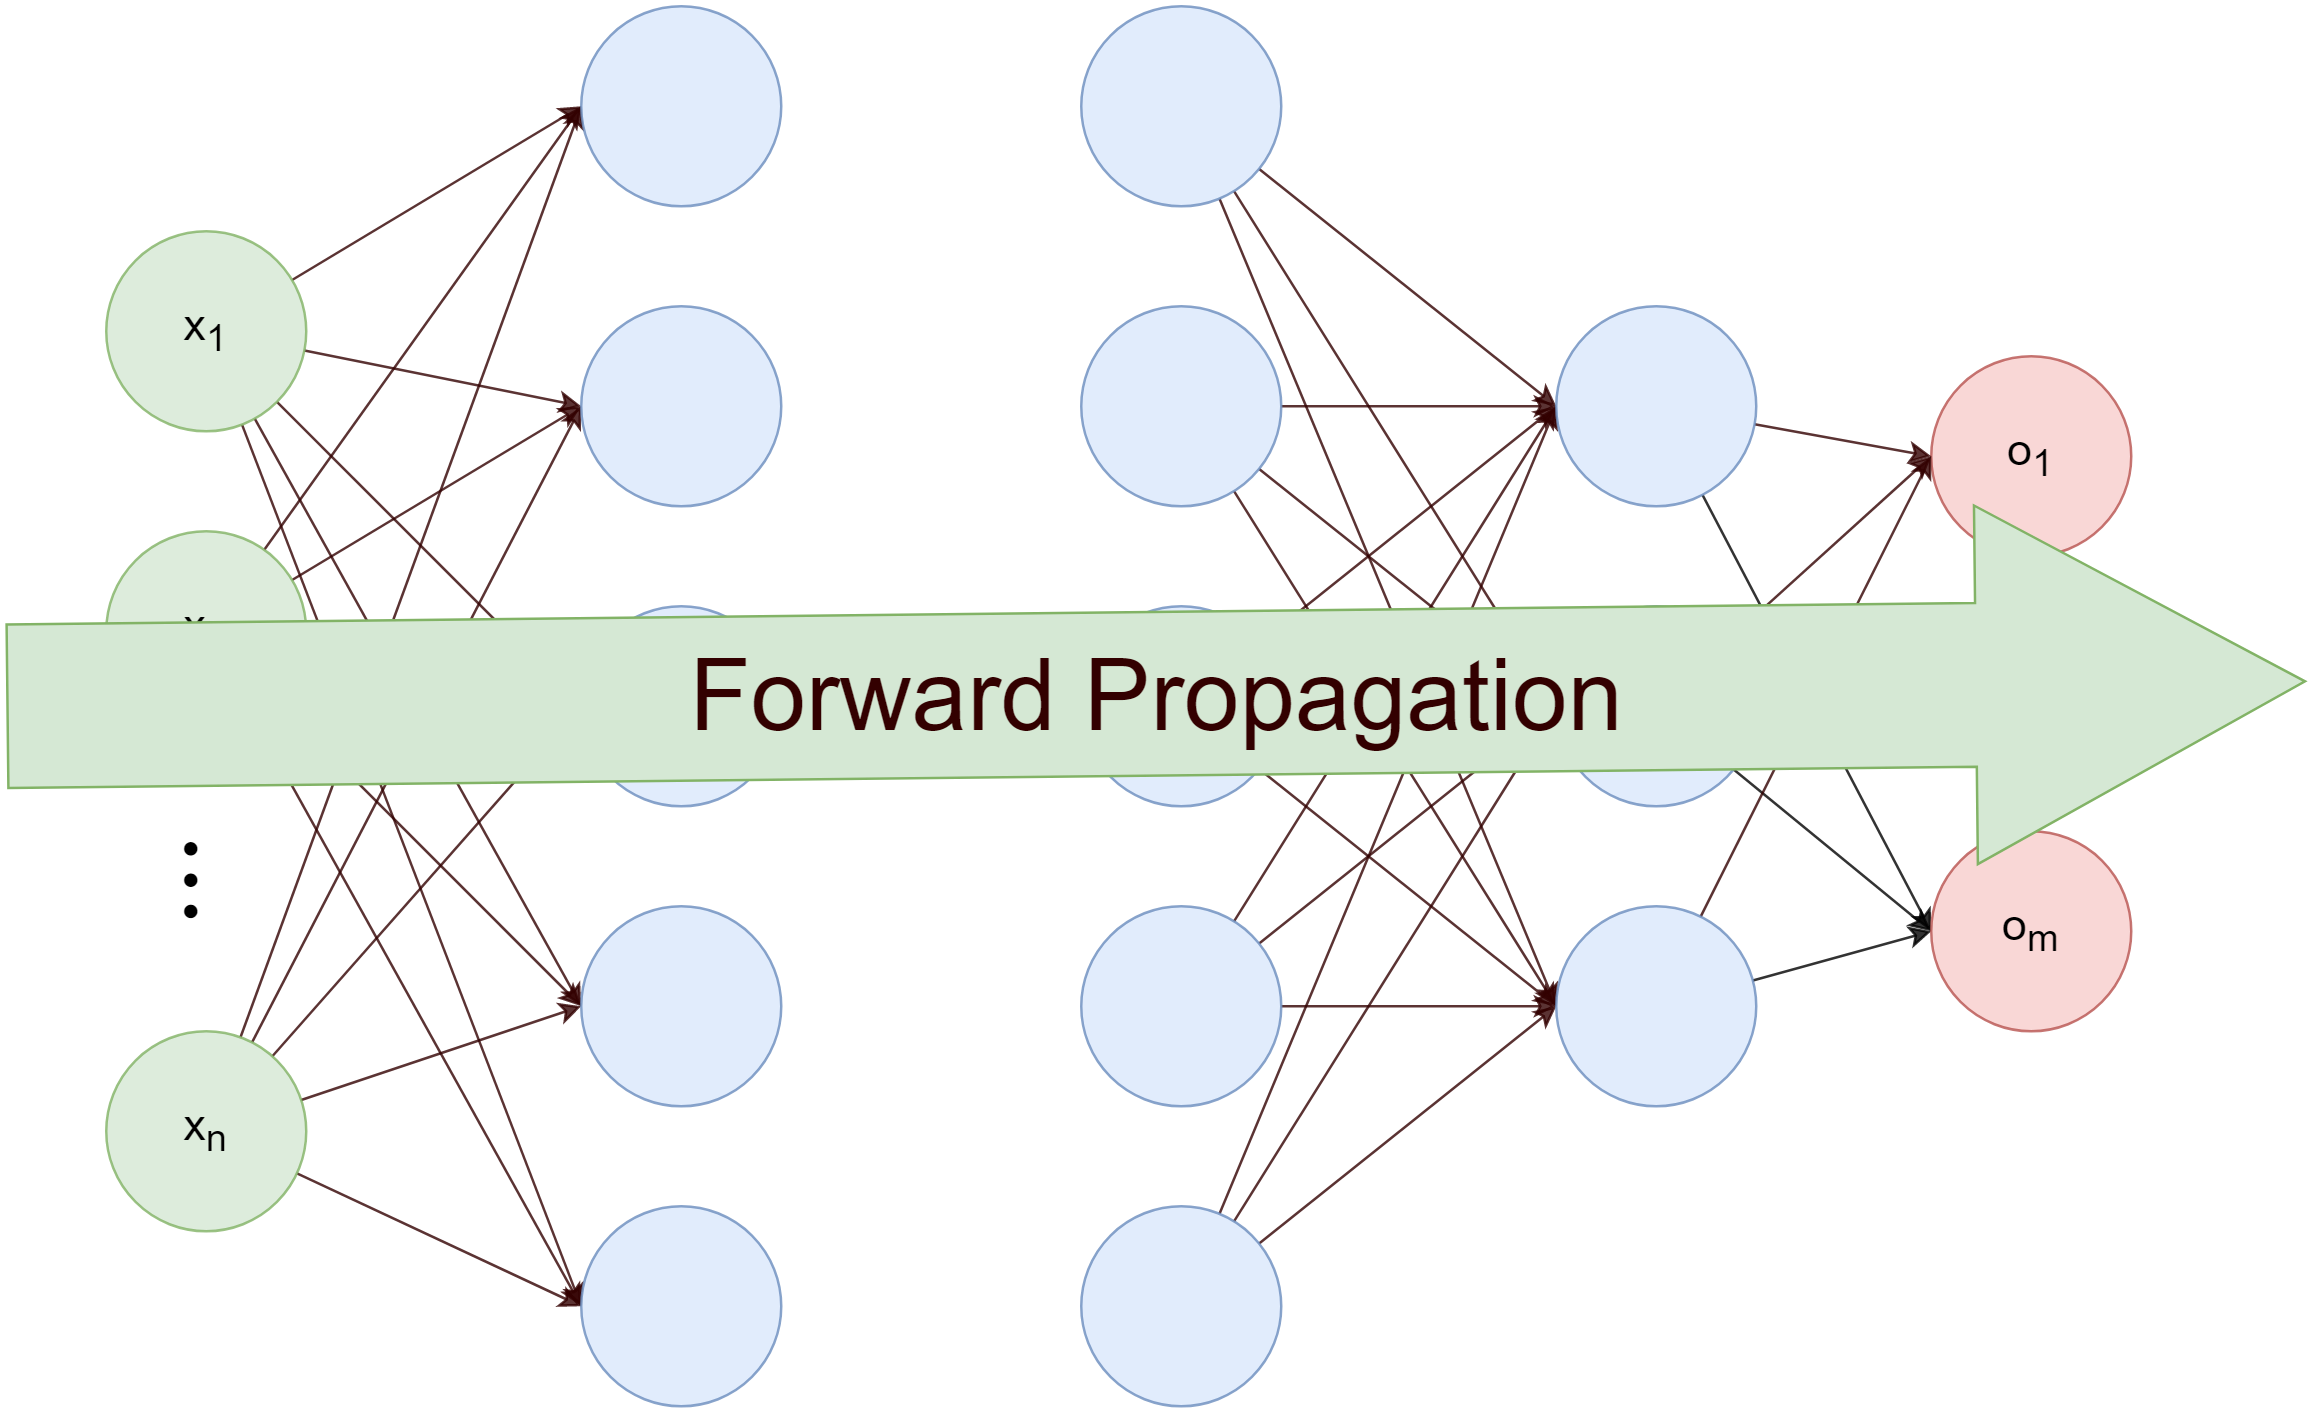
\includegraphics[width=\textwidth]{Figs/forward_propagation.png}
			\caption{Forward pass}
		\end{subfigure}
		\begin{subfigure}[b]{0.3\textwidth}
			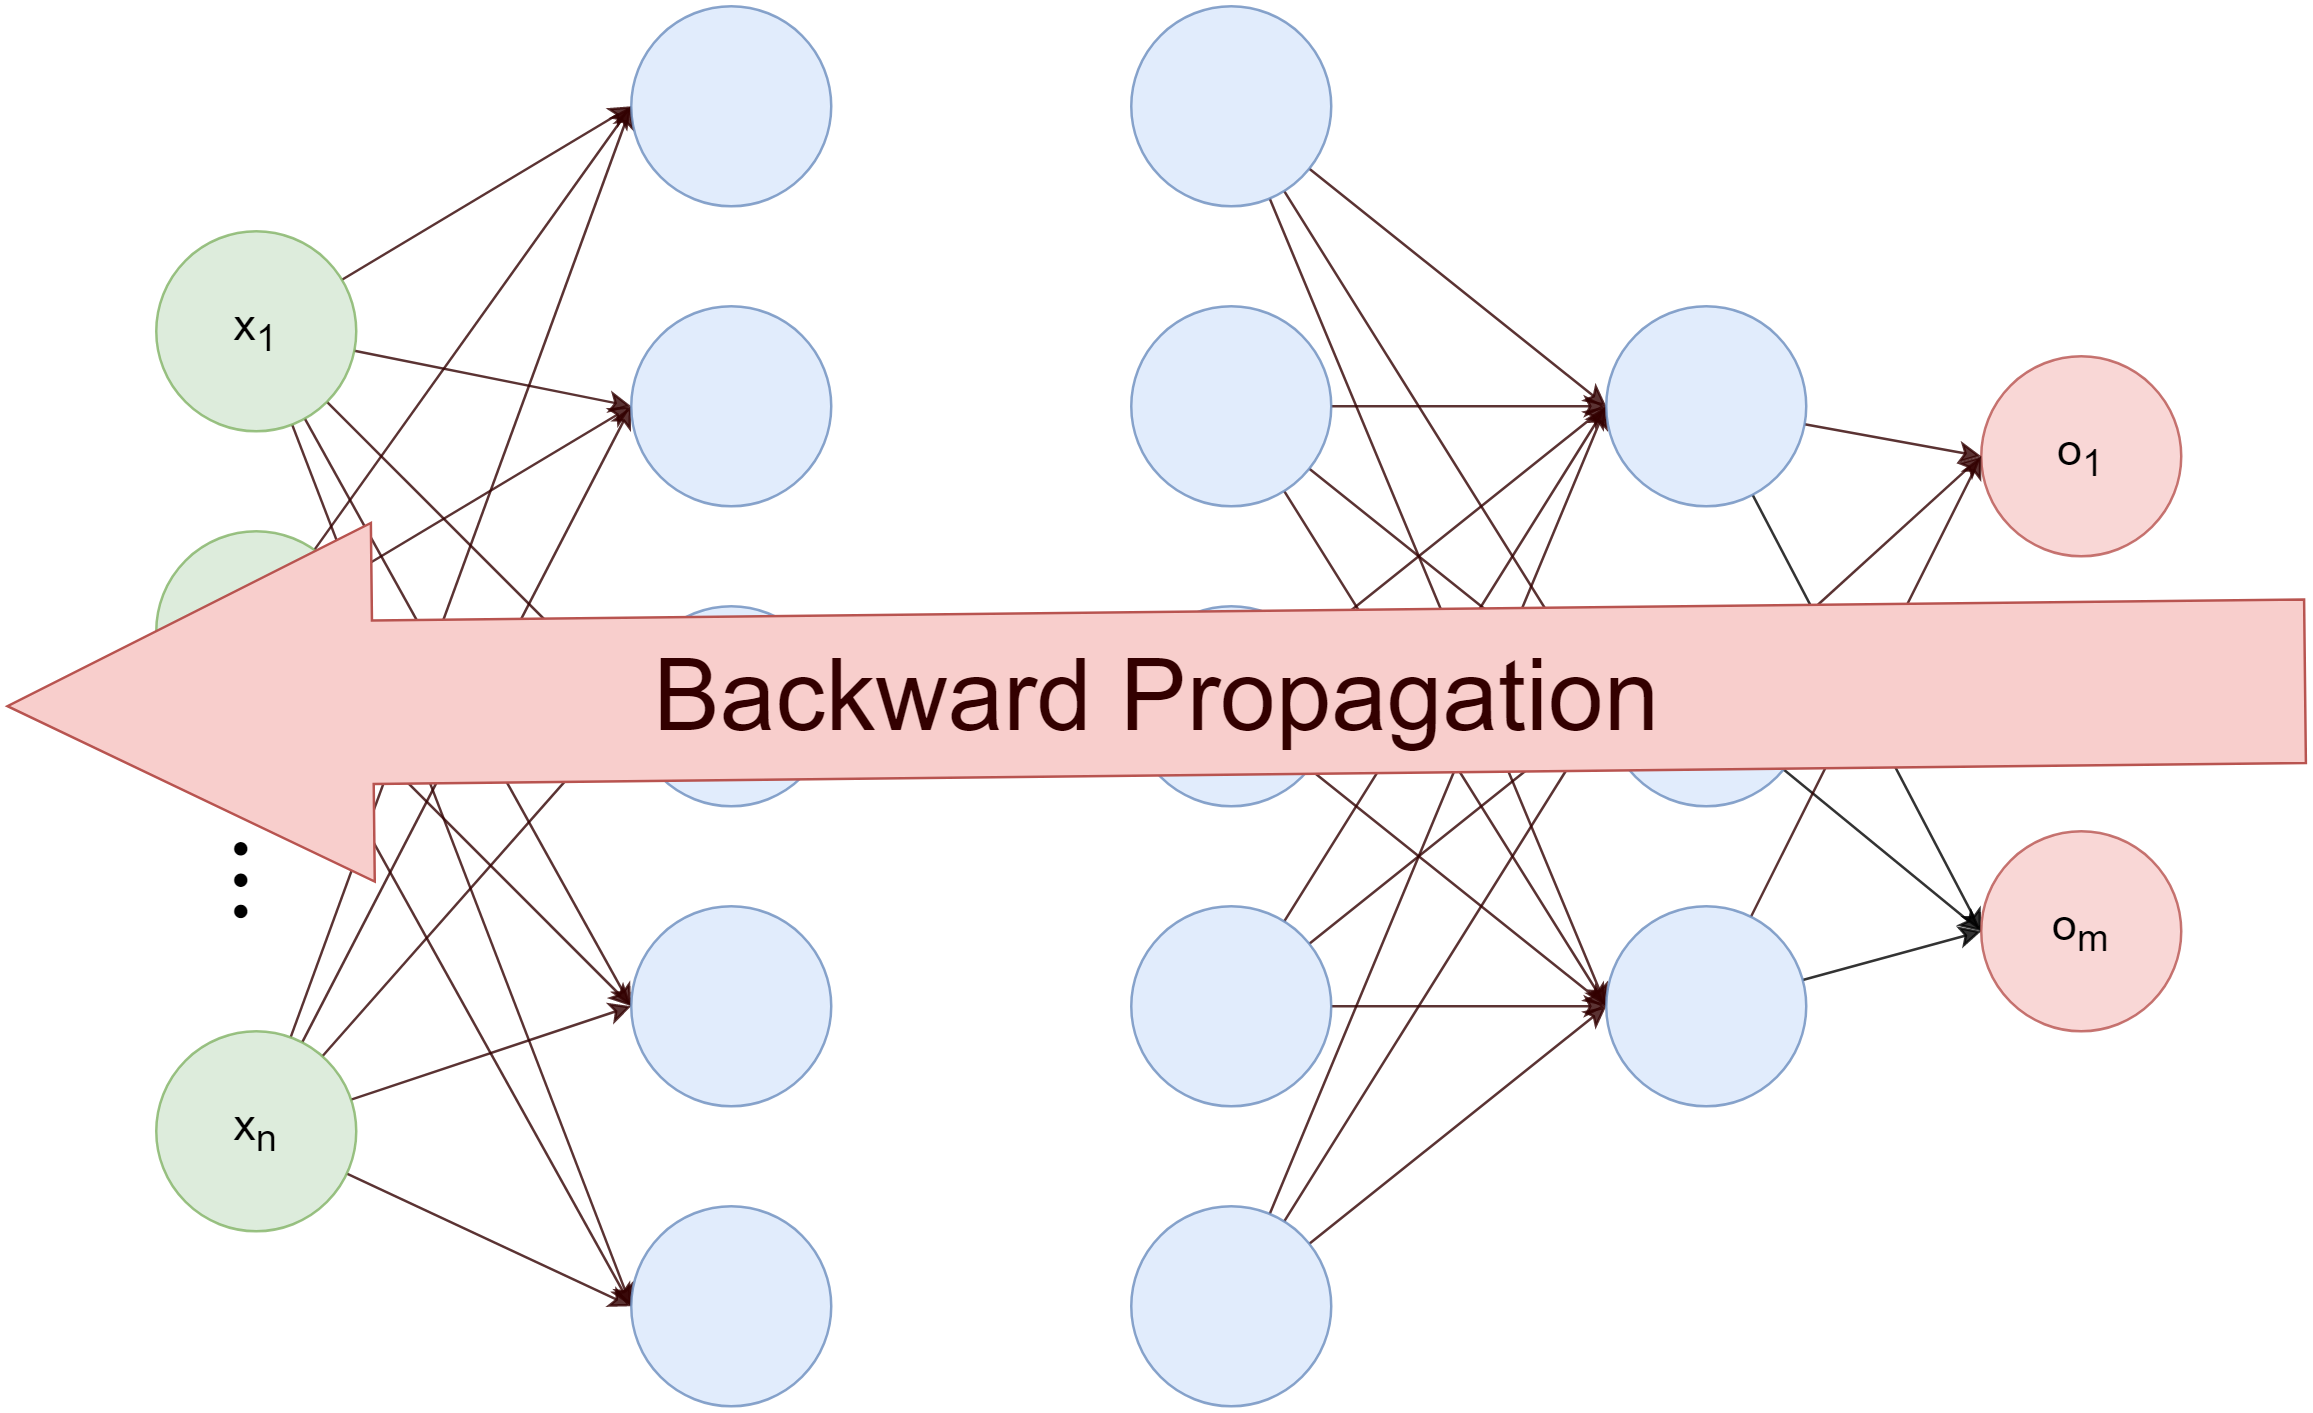
\includegraphics[width=\textwidth]{Figs/backward_propagation.png}
			\caption{Backward pass}
		\end{subfigure}
		\begin{subfigure}[b]{0.28\textwidth}
			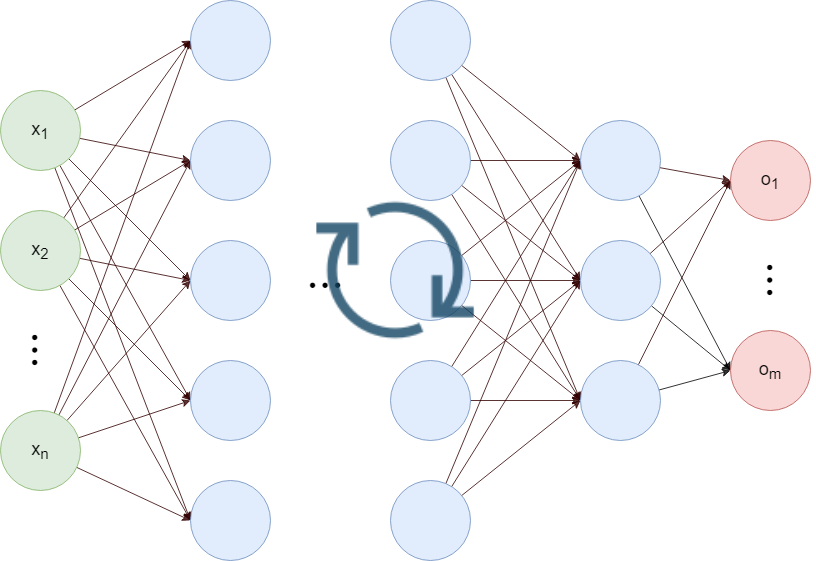
\includegraphics[width=\textwidth]{Figs/update_phase.png}
			\caption{Update parameters}
		\end{subfigure}
	\end{figure}
\end{frame}

\begin{frame}{Learning MLPs}
	\begin{itemize}
		\item Let's define the learning problem more formal:
		\begin{itemize}
			\item $\{(x^{(i)}, y^{(i)})\}_{i=1}^{n}$: dataset
			\item $f$: network
			\item $W$: all weights and biases of the network ($W^{[l]}$ and $\bm{b}^{[l]}$ for different $l$)
			\item $L$: loss function
		\end{itemize}
		\medskip
		\item We want to find $W^{\ast}$ which minimizes following cost function:
		\[
		\mathcal{J}(W) = \sum_{i=1}^{n} L\left(f(x^{(i)}; W), y^{(i)}\right)
		\]
		\item We are going to use gradient descent, so we need to find $\nabla_W \mathcal{J}$.
	\end{itemize}
\end{frame}

\begin{frame}{Forward Propagation}
	\begin{itemize}
		\item First of all we need to find loss value.
		\item It only requires to know the inputs of each neuron.
	\end{itemize}
	\begin{figure}[H]
		\centering
		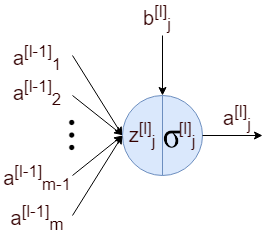
\includegraphics[width=0.3\textwidth]{Figs/forward_pass.png}
		\caption{$a^{[l]}_j = \sum_{i=1}^m W^{[l]}_{ij}a^{[l-1]}_i + b^{[l]}_j$}
	\end{figure}
	\begin{itemize}
		\item So we can calculate these outputs layer by layer.
	\end{itemize}
\end{frame}

\begin{frame}{Forward Propagation}
	\begin{itemize}
		\item After forward pass we will know:
		\begin{itemize}
			\item Loss value
			\item Network output
			\item Middle values
		\end{itemize}
	\end{itemize}
	\begin{figure}[H]
		\centering
		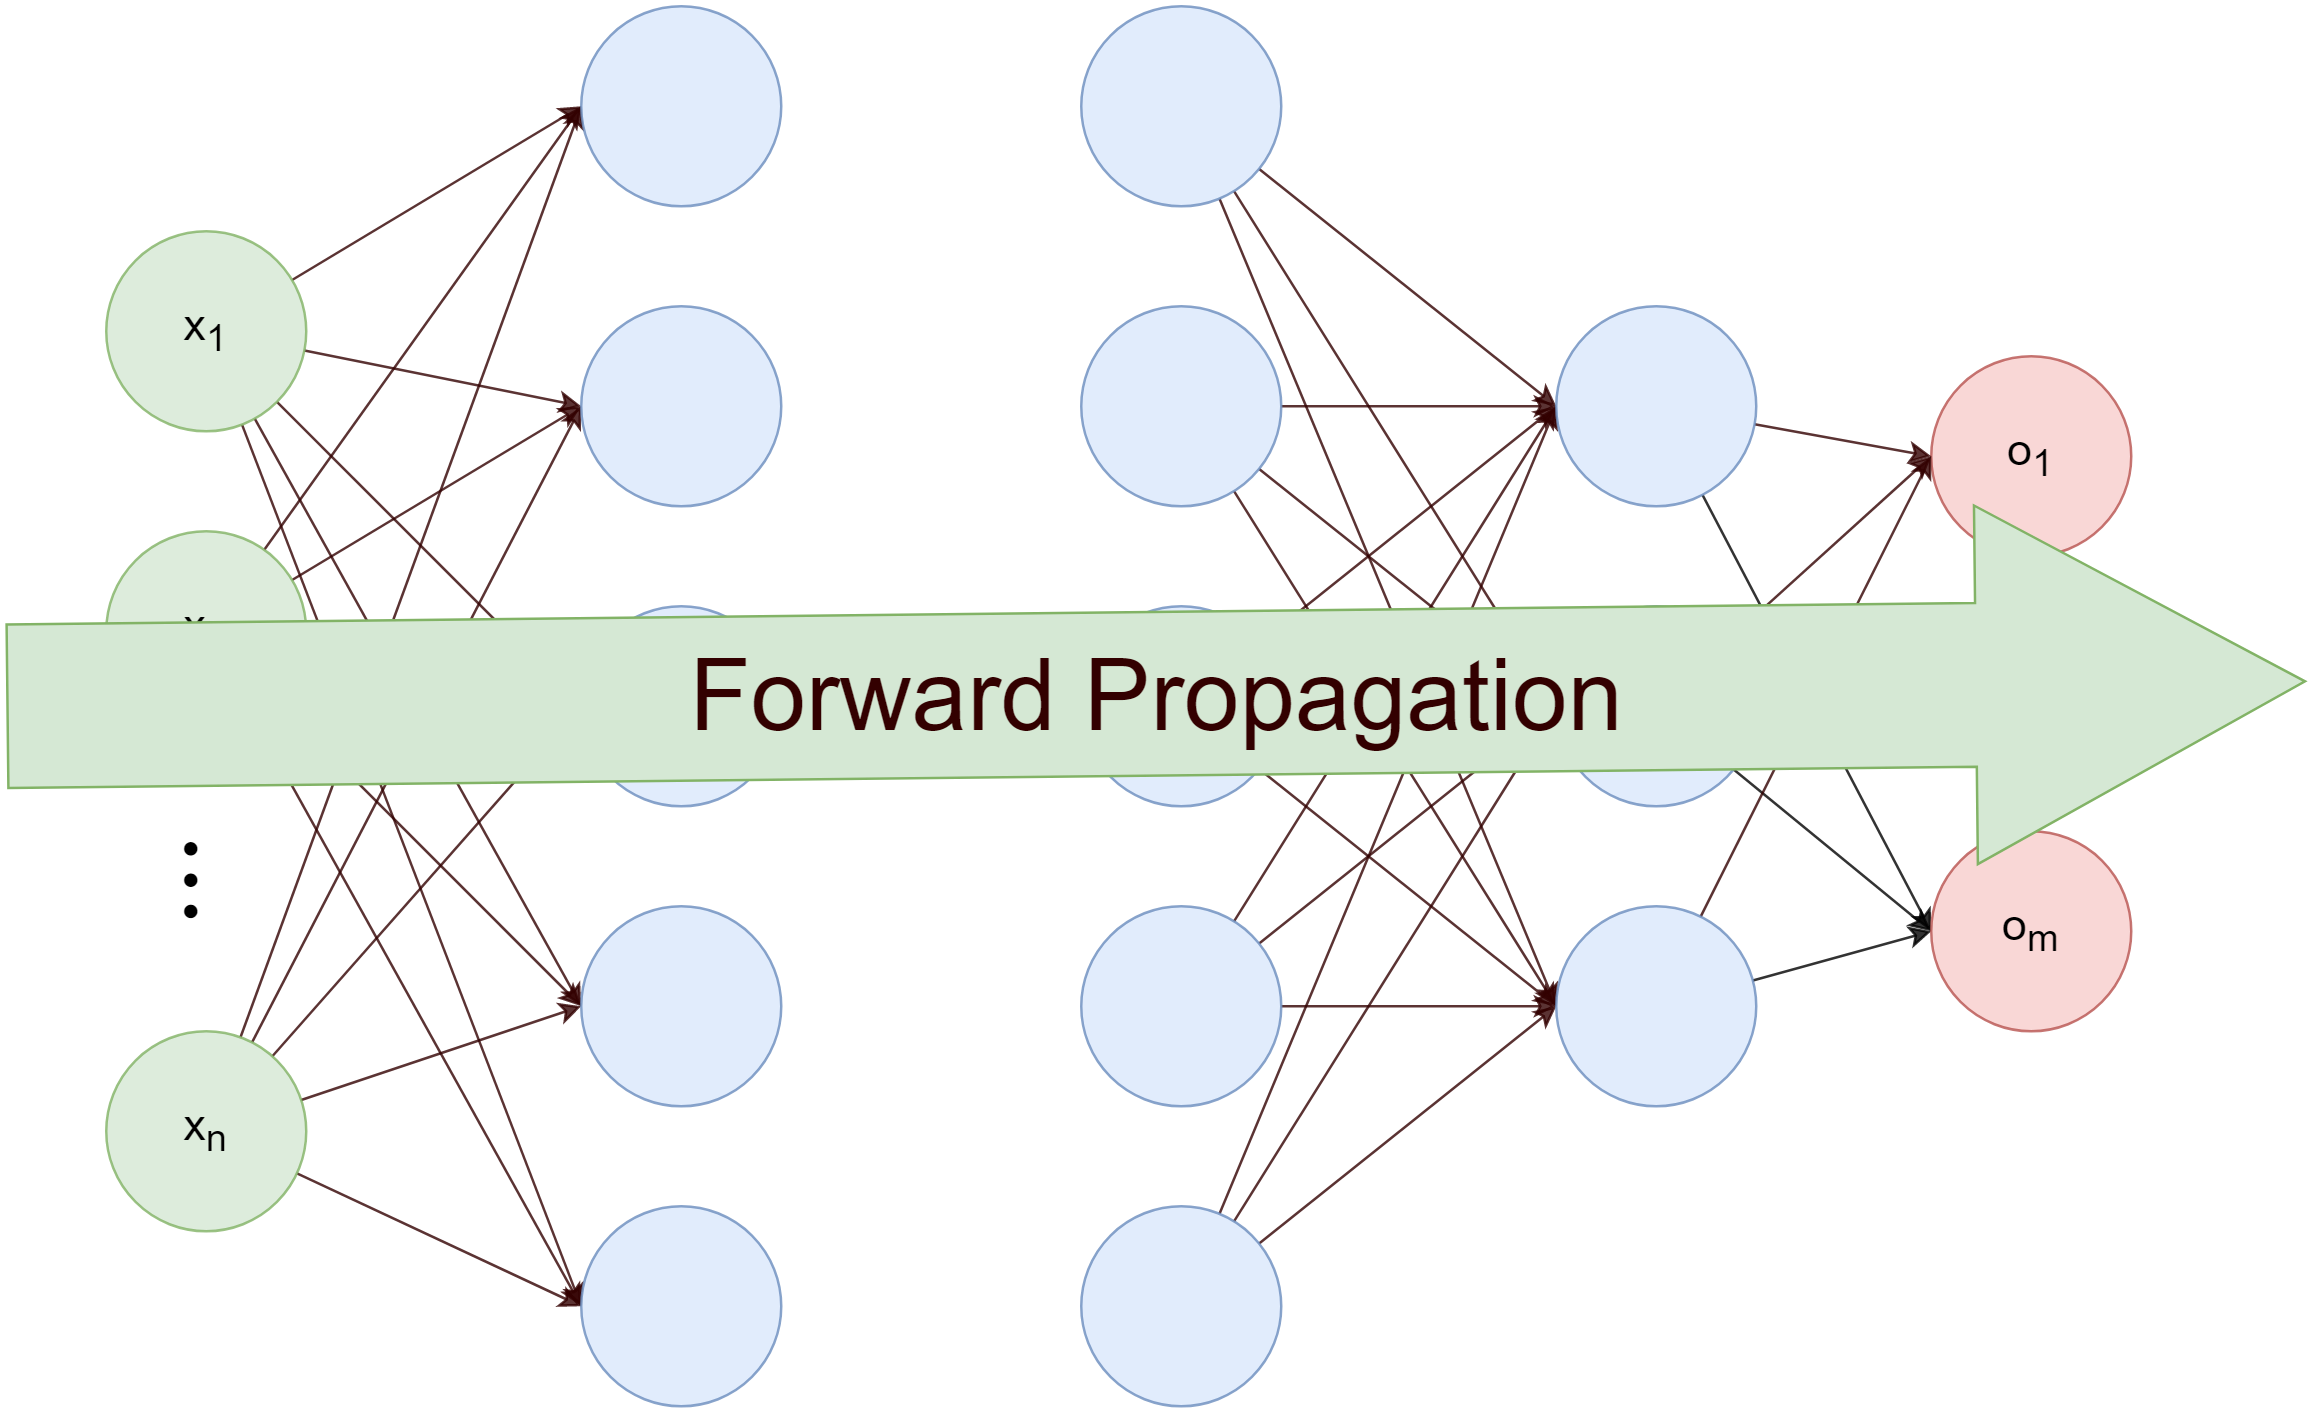
\includegraphics[width=0.5\textwidth]{Figs/forward_propagation.png}
		\caption{Forward pass}
	\end{figure}
\end{frame}

\begin{frame}{Backward Propagation}
	\begin{itemize}
		\item Now we need to calculate $\nabla_W \mathcal{J}$.
		\medskip
		\item First idea:
		\begin{itemize}
			\item Use analytical approach.
			\item Write down derivatives on paper.
			\item Find the close form of $\nabla_W \mathcal{J}$ (if it is possible to do so).
			\item Implement this gradient as a function to work with.
			\medskip
			\medskip
			\item Pros:
			\begin{itemize}
				\item Fast
				\item Exact
			\end{itemize}
			\medskip
			\medskip
			\item Cons:
			\begin{itemize}
				\item Need to rewrite calculation for different architectures
			\end{itemize}
		\end{itemize}
	\end{itemize}
\end{frame}

\begin{frame}{Backward Propagation}
	\begin{itemize}
		\item Second idea:
		\begin{itemize}
			\item Using \tc{keywords}{modular} approach.
			\item Computing the cost function consists of doing many operations.
			\item We can build a computation graph for this calculation.
			\item Each node will represent a single operation.
		\end{itemize}
	\end{itemize}
	\begin{figure}[H]
		\centering
		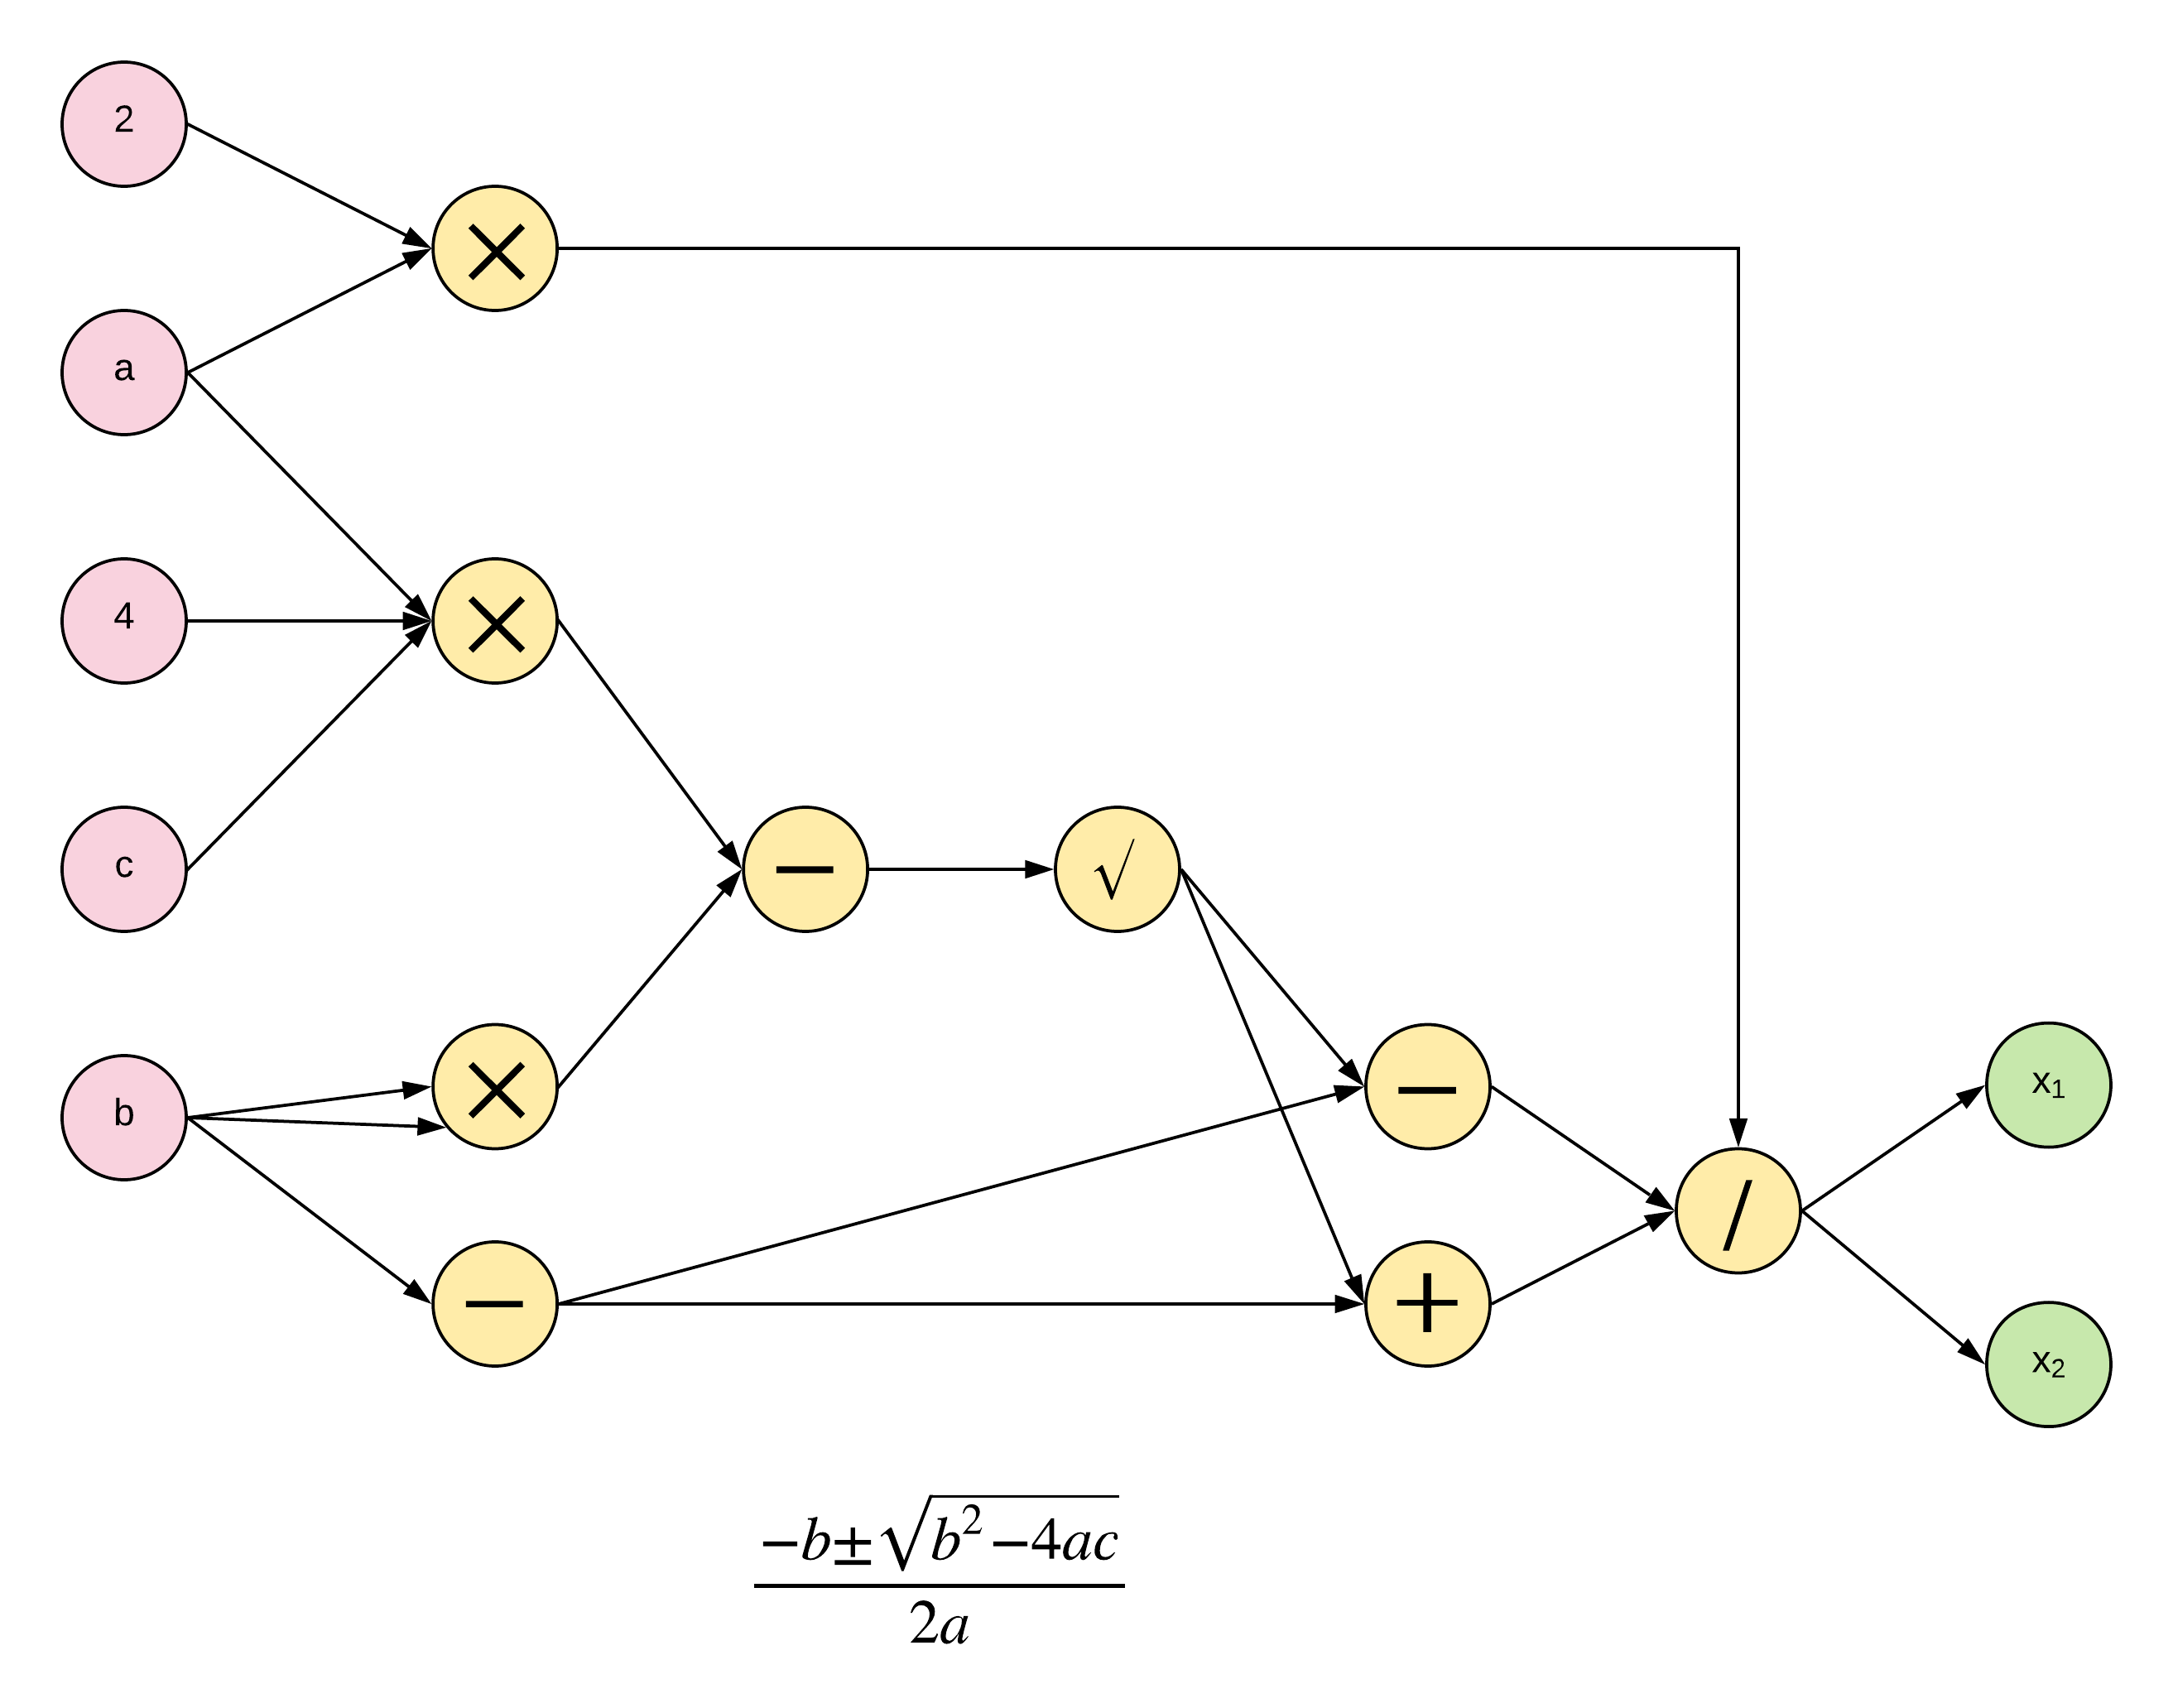
\includegraphics[height=0.5\textheight]{Figs/computational_graph.png}
		\caption{An example of computational graph, \href{https://ekababisong.org/gcp-ml-seminar/tensorflow/}{Source}.}
	\end{figure}
\end{frame}

\begin{frame}{Backward Propagation}
	\begin{itemize}
		\item In this approach if we know how to calculate gradient for single node or module, then we can find gradient with respect to each variables.
		\item Let's say we have a module as follow:
		\begin{figure}[H]
			\centering
			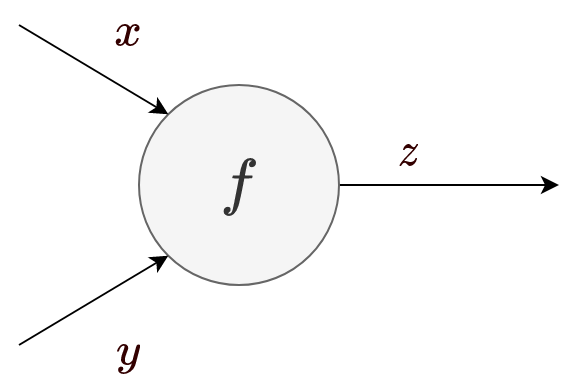
\includegraphics[width=0.35\textwidth]{Figs/module_f.png}
		\end{figure}
		\item It gets $x$ and $y$ as its input and returns $z = f(x, y)$ as its output.
		\item How to calculate derivative of loss with respect to module inputs?
	\end{itemize}
\end{frame}

\begin{frame}{Backward Propagation}
	\begin{itemize}
		\item We know:
		\begin{itemize}
			\item Module output for $x_0$ and $y_0$, let's call it $z_0$.
			\item Gradient of loss with respect to module output at $z_0$, $\left(\frac{\partial L}{\partial z}\right)$.
		\end{itemize}
		\item We want:
		\begin{itemize}
			\item Gradient of loss with respect to module inputs at $x_0$ and $y_0$, $\left(\frac{\partial L}{\partial x}, \frac{\partial L}{\partial y}\right)$.
		\end{itemize}
	\end{itemize}
	\begin{figure}[H]
		\centering
		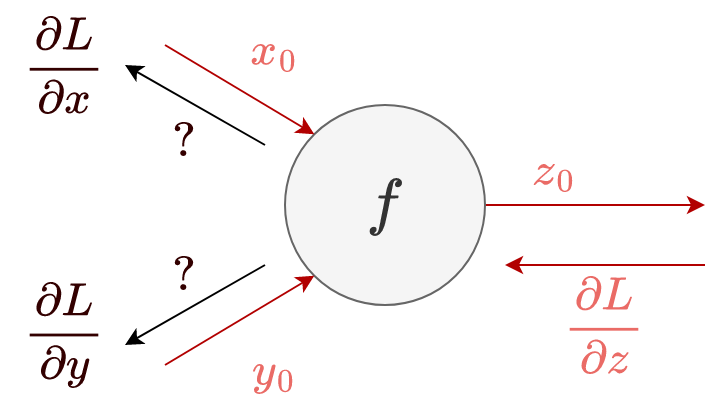
\includegraphics[width=0.4\textwidth]{Figs/module_f_upstream.png}
	\end{figure}
\end{frame}

\begin{frame}{Backward Propagation}
	\begin{itemize}
		\item We can use chain rule to do so.
		\medskip
		\begin{block}{Chain rule:}
			\[
			\left.\begin{aligned}
				& z = f(x, y)\\
				& L = L(z)
			\end{aligned}\right\}\quad\implies\quad \frac{\partial L}{\partial x} = \frac{\partial L}{\partial z}\times \frac{\partial z}{\partial x} 
			\]
		\end{block}
	\end{itemize}
	\begin{figure}[H]
		\centering
		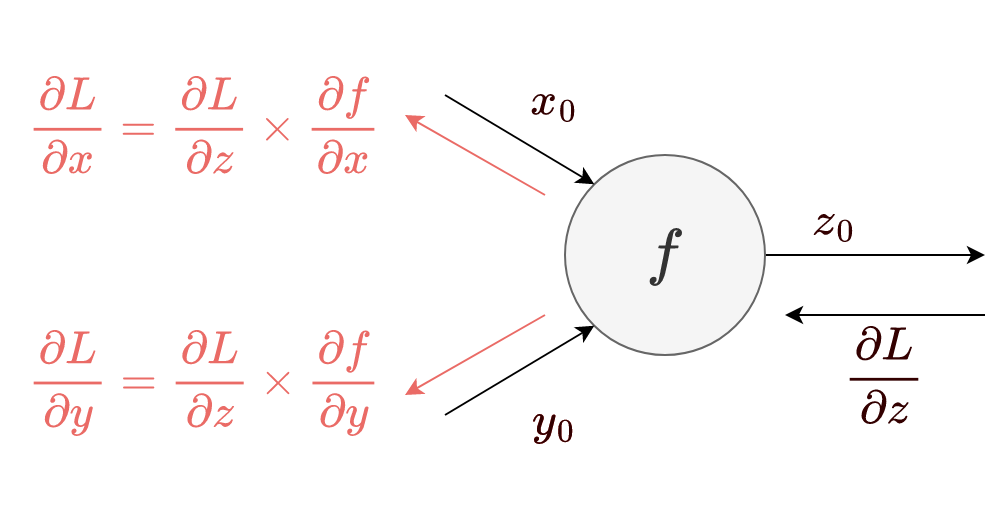
\includegraphics[width=0.6\textwidth]{Figs/module_f_downstream.png}
	\end{figure}
\end{frame}



\begin{frame}{Backward Propagation}
	\begin{itemize}
		\item So after backward propagation we will have:
		\begin{itemize}
			\item Gradient of loss with respect to each parameter.
			\item We can apply gradient descent to update parameters.
		\end{itemize}
	\end{itemize}
	\begin{figure}[H]
		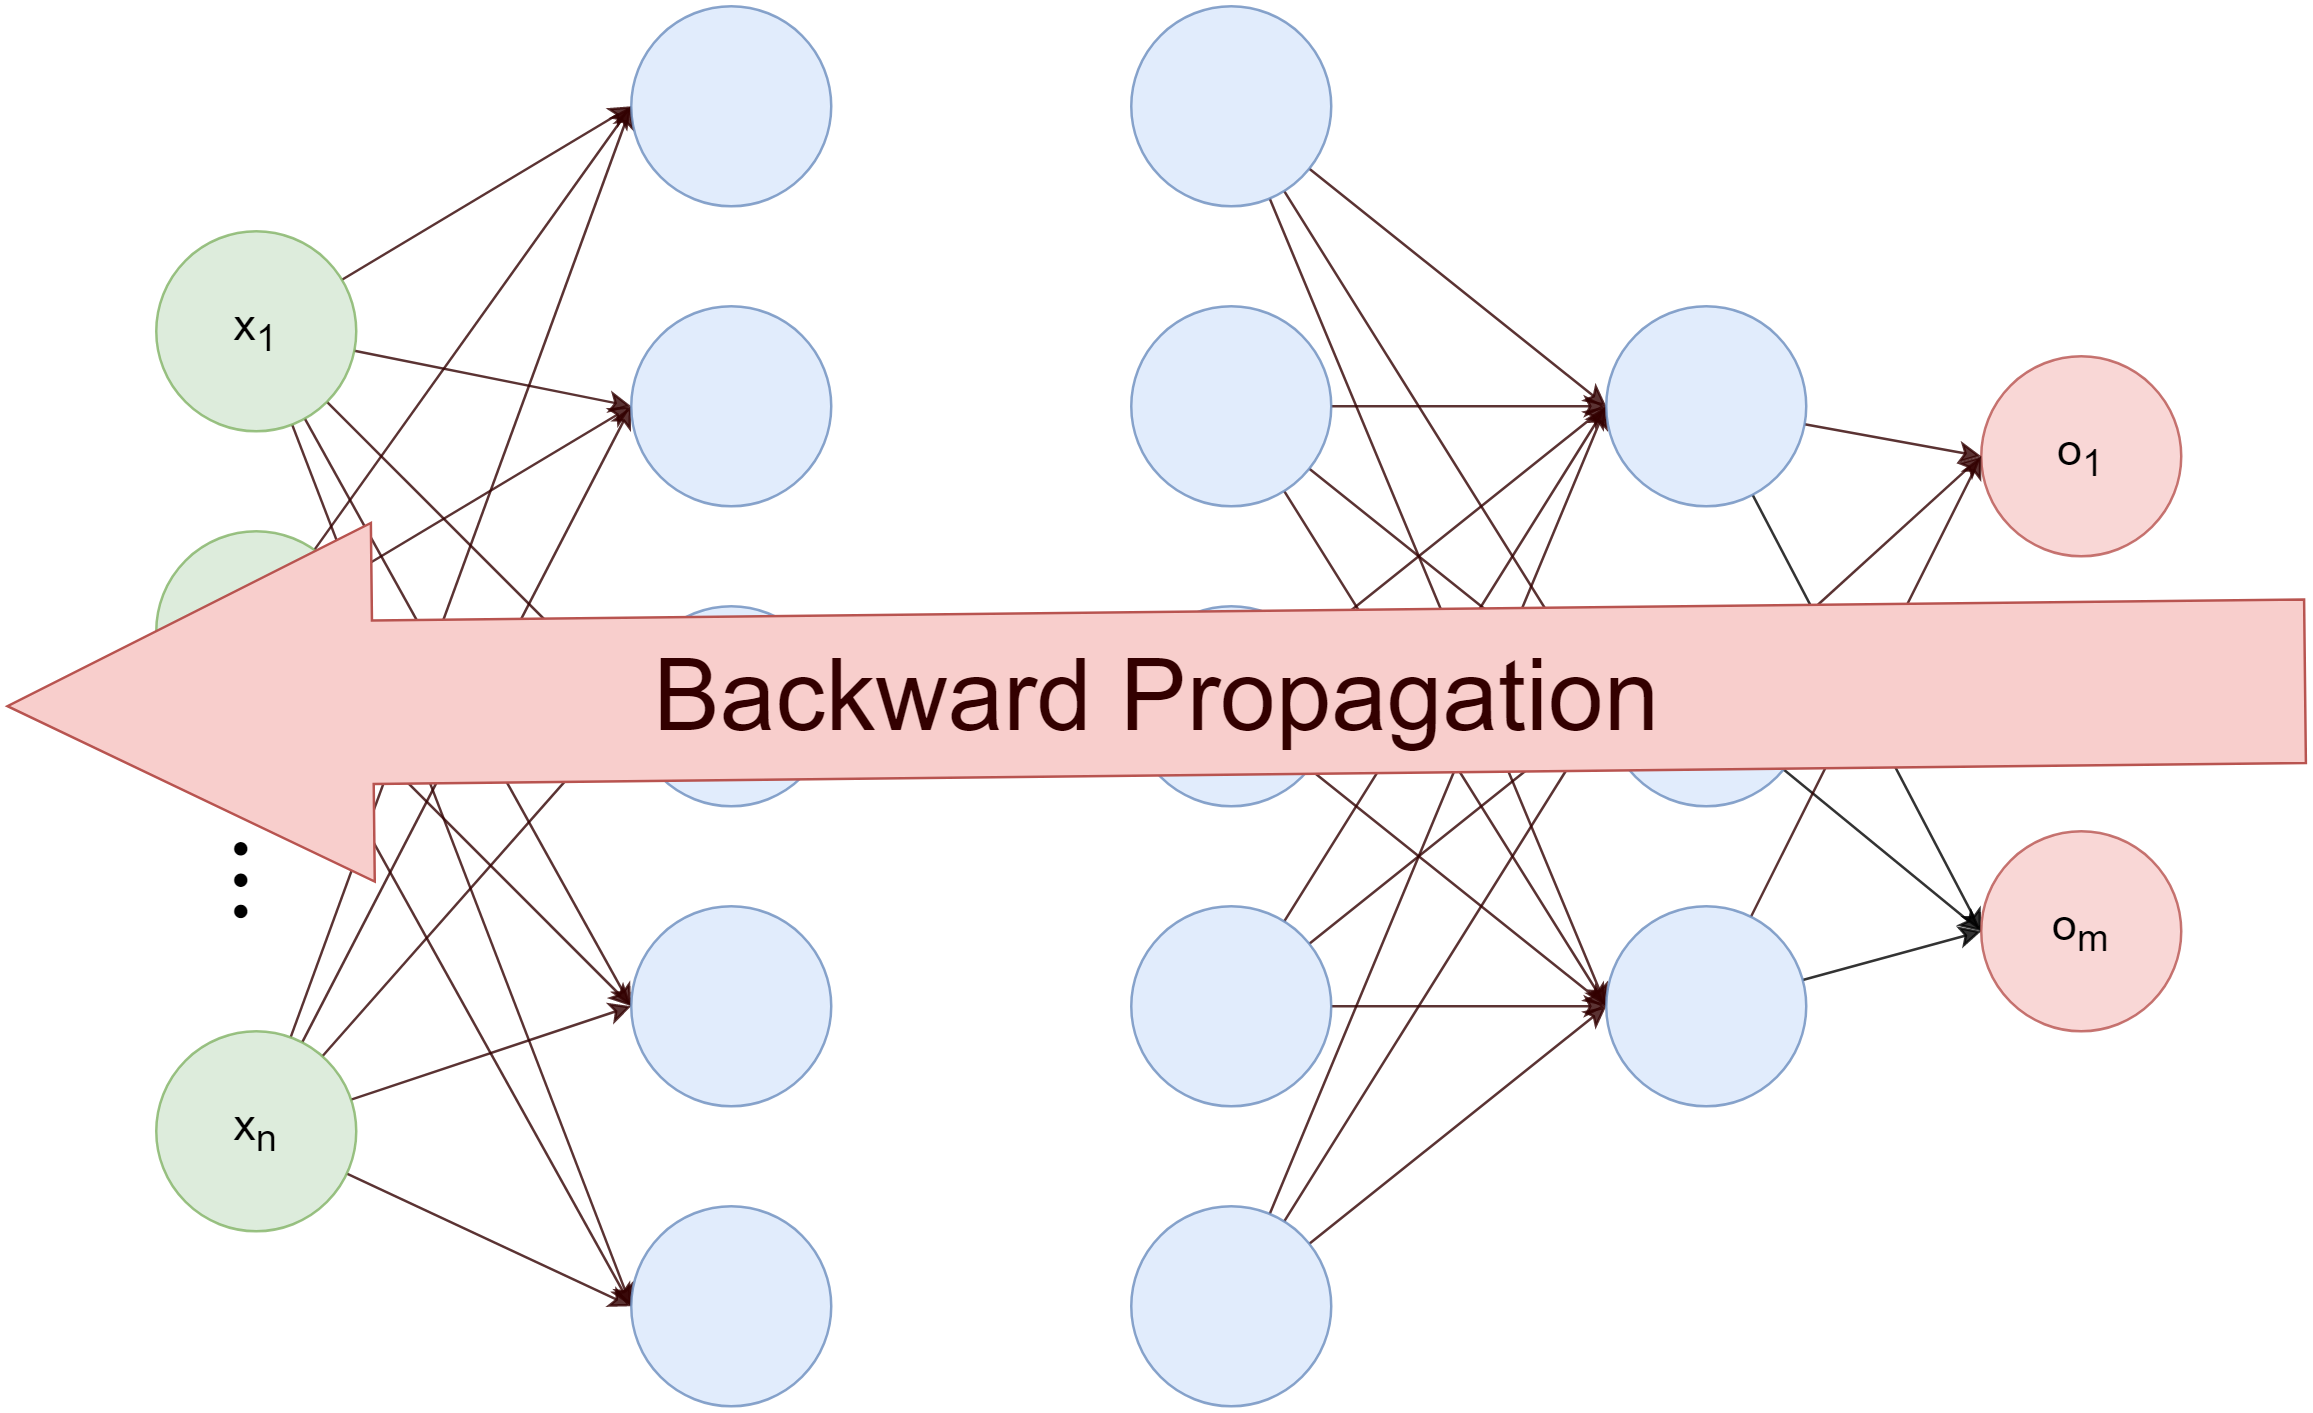
\includegraphics[width=0.5\textwidth]{Figs/backward_propagation.png}
		\caption{Backward pass}
	\end{figure}
\end{frame}


%%%%%%%%%%%%%%%%%%%%%%%%%%[Gradient Descent]%%%%%%%%%%%%%%%%%%%%%%%%%%%%%%%%%%%%%%%%%%%
\section{Gradient Descent}
\begin{frame}{Loss functions}
	\begin{itemize}
		\item So far you got familiar with gradient-based optimization.
		\item If $\bm{g} = \nabla_{\bm{\theta}} \mathcal{J}$, then we will update parameters with this simple rule:
		\[
		\bm{\theta} \gets \bm{\theta} - \eta\bm{g}
		\]
		% 	\item[]
		\item But there is one question here, how to compute $\bm{g}$?
		\item Based on how we calculate $\bm{g}$ we will have different types of gradient descent:
		\begin{itemize}
			\item Batch Gradient Descent
			\item Stochastic Gradient Descent
			\item Mini-Batch Gradient Descent
		\end{itemize}
	\end{itemize}
\end{frame}

\begin{frame}{Various GD types}
	\begin{block}{Recap:}
		Training cost function ($\mathcal{J}$) over a dataset usually is the average of loss function ($\mathcal{L}$) on entire training set, so for a dataset $\mathcal{D}=\{d_i\}_{i=1}^n$ we have:
		\[
		\mathcal{J}(\mathcal{D}) = \frac{1}{n} \sum_{i=1}^{n} \mathcal{L}(d_i; \bm{\theta})
		\]
		For example:
		\begin{equation*}
			H(p, q)=-\frac{1}{m} \sum_{i=1}^m\sum_{j=1}^{k} y_j^{(i)} \log (p(y_j^{(i)}))
		\end{equation*}
		\begin{equation*}
			\text{MSE}(y, \hat{y}) = \frac{1}{m}\sum_{i=1}^{m}(y_i-\hat{y}_i)^2
		\end{equation*}
		\begin{equation*}
			\text{MAE}(y, \hat{y}) = \frac{1}{m}\sum_{i=1}^{m}|(y_i-\hat{y}_i)|
		\end{equation*}
	\end{block}
\end{frame}

\begin{frame}{Various GD types: Batch Gradient Descent}
	\begin{itemize}
		\item In this type we use \tc{keywords}{entire training set} to calculate gradient.
		\begin{block}{Batch Gradient:}
			\[
			\bm{g} = \frac{1}{n}\sum_{i=1}^n \nabla_{\bm{\theta}} \mathcal{L}(d_i, \bm{\theta})
			\]
		\end{block}
		\item[]
		\item Using this method with very large training set:
		\begin{itemize}
			\item Your data can be too large to process in your memory.
			\item It requires a lot of processing to compute gradient for all samples.
		\end{itemize}
		\item Using exact gradient may lead us to local minima.
		\item Moving noisy may help us get out of this local minimas.
	\end{itemize}
\end{frame}

\begin{frame}{Various GD types: Batch Gradient Descent}
	\begin{figure}[H]
		\centering
		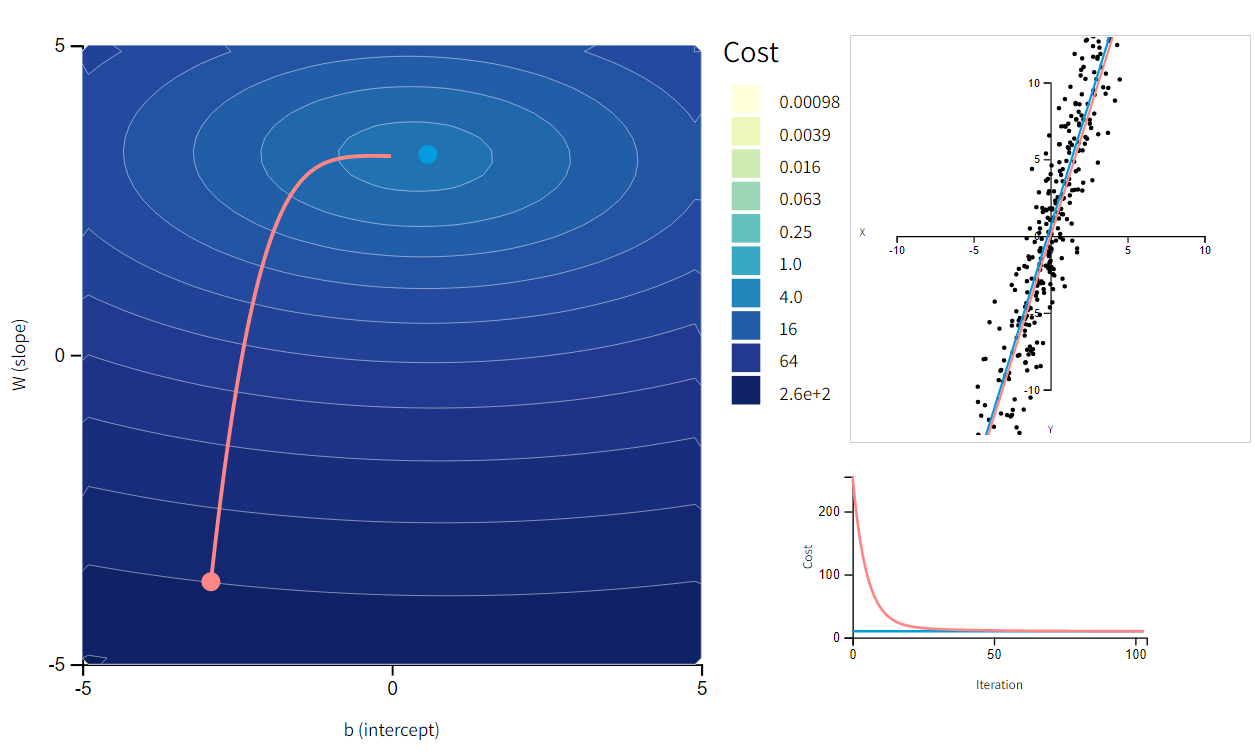
\includegraphics[width=0.8\textwidth]{Figs/bgd.png}
		\caption{Optimization of parameters using BGD. Movement is very smooth \cite{katanforoosh-kunin-opt}.}
	\end{figure} 
\end{frame}

\begin{frame}{Various GD types: Stochastic Gradient Descent}
	\begin{itemize}
		\item Instead of calculating exact gradient, we can estimate it using our data.
		\item This is exactly what SGD does, it estimates gradient using \tc{keywords}{only single data point}.
		\begin{block}{Stochastic Gradient:}
			\[
			\hat{\bm{g}} = \nabla_{\bm{\theta}} \mathcal{L}(d_i, \bm{\theta})
			\]
		\end{block}
		\item[]
		\item As we use an approximation of gradient, instead of gently decreasing, the cost function will bounce up and down and decrease only on average.
		\item This method is really computationally efficient cause we only need to calculate gradient for one point per iteration. 
	\end{itemize}
\end{frame}

\begin{frame}{Various GD types: Stochastic Gradient Descent}
	\begin{figure}[H]
		\centering
		\includegraphics[width=0.8\textwidth]{Figs/sgd.png}
		\caption{Optimization of parameters using SGD. As we expect, the movement is not that smooth \cite{katanforoosh-kunin-opt}.}
	\end{figure} 
\end{frame}

\begin{frame}{Various GD types: Mini-Batch Gradient Descent}
	\begin{itemize}
		\item In this method we still use estimation idea But use \tc{keywords}{a batch of data} instead of one point.
		\begin{block}{Mini-Batch Gradient:}
			\[
			\hat{\bm{g}} = \frac{1}{|\mathcal{B}|} \sum_{d\in\mathcal{B}} \nabla_{\bm{\theta}} \mathcal{L}(d, \bm{\theta}), \quad \mathcal{B} \subset \mathcal{D}
			\]
		\end{block}
		\item[]
		\item This is a better estimation than SGD.
		\item With this way we can get a performance boost from hardware optimization, especially when using GPUs.
		\item Batch size ($|\mathcal{B}|$) is a hyperparameter you need to tune.
	\end{itemize}
\end{frame}

\begin{frame}{Various GD types: Mini-Batch Gradient Descent}
	\begin{figure}[H]
		\centering
		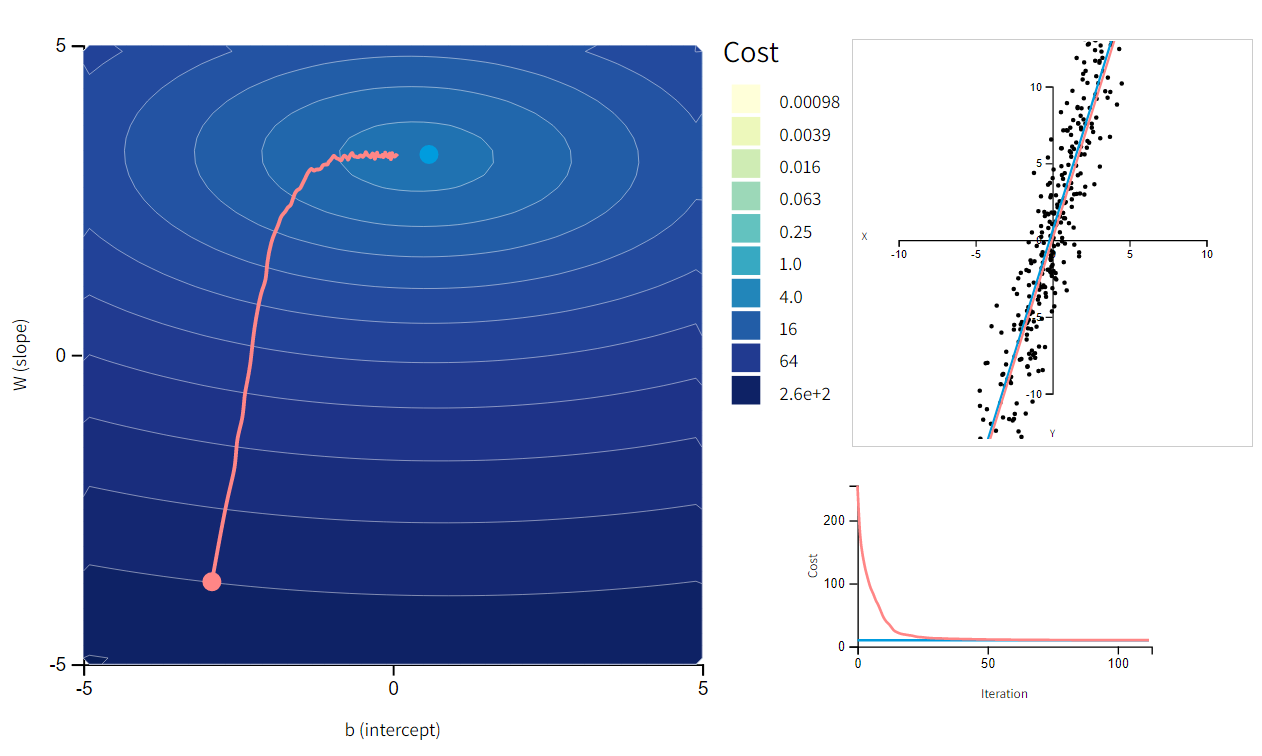
\includegraphics[width=0.8\textwidth]{Figs/mbgd.png}
		\caption{Optimization of parameters using MBGD. The movement is much smother than SGD and behaves like BGD \cite{katanforoosh-kunin-opt}.}
	\end{figure} 
\end{frame}


\begin{frame}{Various GD types}
	\begin{itemize}
		\item So we got familiar with different types of GD.
		\begin{itemize}
			\item[\color{darkgreen}$\checkmark$] Batch Gradient Descent (BGD)
			\item[\color{darkgreen}$\checkmark$] Stochastic Gradient Descent (SGD)
			\item[\color{darkgreen}$\checkmark$] Mini-Batch Gradient Descent (MBGD)
		\end{itemize}
		\item[]
		\item[]
		\item The most recommended one is MBGD, because it is computationally efficient.
		\item Choosing the right batch size is important to ensure convergence of the cost function and parameter values, and to the generalization of your model.
	\end{itemize}
\end{frame}
%%%%%%%%%%%%%%%%%%%%%%%%%%%%%%%%% [training MLPs] %%%%%%%%%%%%%%%%%%%%%%%%%%%%%%%%%%%%%%%%
\section{Training MLPs}
\begin{frame}{Training MLPs}
	\begin{itemize}
		\item So far we have learned about how MLPs work and how to update their parameters in order to perform better.
		\item But training MLPs is not that easy.
		\item You will face several different challenges in this procedure.
		\item In this section we will talk about this challenges and how to solve them.
	\end{itemize}
\end{frame}


%%%%%%%%%%%%%%%%%%%%%%%%[Vanishing Exploding]%%%%%%%%%%%%%%%%%%%%%%%%
\begin{frame}{Vanishing/Exploding Gradient}
	\begin{itemize}
		\item The backpropagation algorithm propagates the error gradient while proceeding from the output layer to the input layer. The issue here is the magnitude of the cost function gradients through the layers... 
	\end{itemize}
	\begin{figure}
		\centering
		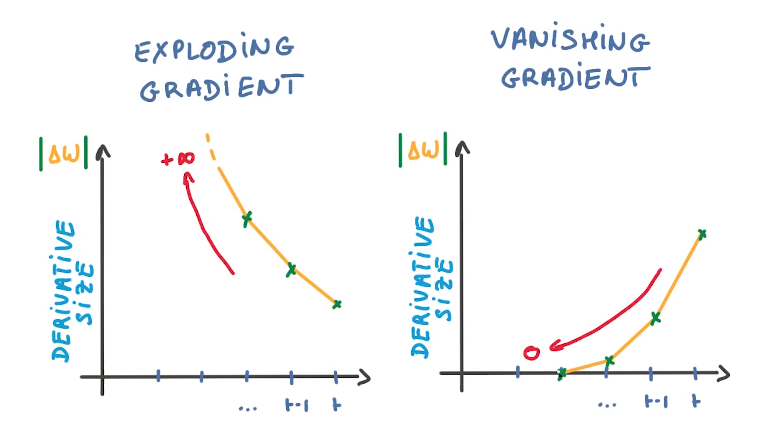
\includegraphics[width=8cm, height=4cm]{Figs/van_2.png}
		\caption{Vanishing/Exploding Gradient, \href{https://medium.com/@ayushch612/vanishing-gradient-and-exploding-gradient-problems-7737c0aa535f}{Source}}
	\end{figure}
\end{frame}

\begin{frame}{Vanishing/Exploding Gradient}
	\begin{itemize}
		\item Vanishing
		\begin{itemize}
			\item Gradients often get smaller as the algorithm progresses down. As a result, gradient descent updates do not effectively change the weights of the lower layer connections, and training never converges.
			\medskip
			\item Make learning slow especially of front layers in the network.
			\medskip
		\end{itemize}
		\item Exploding
		\begin{itemize}
			\item Gradients can get bigger and bigger, so there are very large weight updates at many levels, causing the algorithm to diverge.
			\medskip
			\item The model is not learning much on the training data therefore resulting in a poor loss.
			\medskip
		\end{itemize}
	\end{itemize}
\end{frame}


%%%%%%%%%%%%%%%%%%%%%%%%%%%%%%%%[Weight Initialization]%%%%%%%%%%%%%%%%%%%%%%%%%%%%%%%%%%%
\begin{frame}{Weight Initialization}
	\begin{itemize}
		\item Is initialization really necessary?
		\item What are the impacts of initialization?
		\item A bad initialization may increase convergence time or even make optimization diverge.
		\item How to initialize?
		\begin{itemize}
			\item Zero initialization
			\item Random initialization
		\end{itemize}
	\end{itemize}
	\begin{figure}[H]
		\centering
		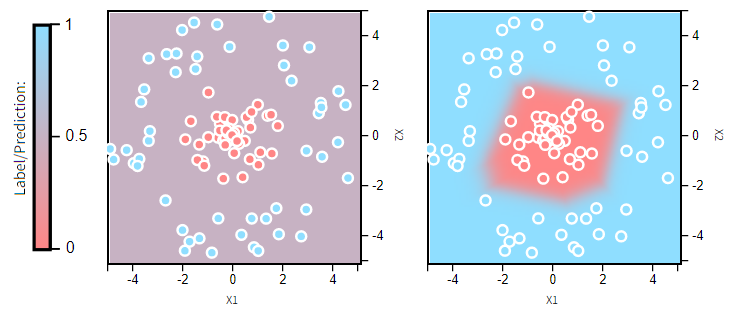
\includegraphics[width=0.65\textwidth]{Figs/wi-crucial.png}
		\caption{The output of a three layer network after about 600 epochs. (left) using a bad\\ initialization method and (right) using an appropriate initialization \cite{katanforoosh-kunin}.}
	\end{figure}
\end{frame}

\begin{frame}{Weight Initialization: Zero Initialization}
	\begin{block}{Zero Initialization method:}
		\[
		\begin{cases}
			W^{[l]} = \bm{0},\\
			b^{[l]} = \bm{0}
		\end{cases}
		\]
	\end{block}
	\begin{itemize}
		\item[]
		\item[]
		\item Simple but perform very poorly. (why?)
		\item Zero initialization will lead each neuron to learn the same feature
		\item This problem is known as network {\color{red}failing to break symmetry}
		\item In fact any constant initialization suffers from this problem.
	\end{itemize}
\end{frame}

\begin{frame}{Weight Initialization: Random Initialization}
	\begin{itemize}
		\item To use randomness in our initialization we can use uniform or normal distribution:
		\medskip
		\item[]\begin{block}{General Uniform Initialization:}
			\[
			\begin{cases}
				W^{[l]} \sim U(-r, +r),\\
				b^{[l]} = 0
			\end{cases}
			\]
		\end{block}
		\item[]\begin{block}{General Normal Initialization:}
			\[
			\begin{cases}
				W^{[l]} \sim \mathcal{N}(\mu=0, \sigma^2),\\
				b^{[l]} = 0
			\end{cases}
			\]
		\end{block}
		\item But this is really crucial to choose $r$ or $\sigma$ properly.
	\end{itemize}
\end{frame}

\begin{frame}{More On Weight Initialization}
	\begin{itemize}
		\item To read more about different weight initialization methods and deepen your understanding about how it can affect your network, visit \href{https://www.deeplearning.ai/ai-notes/initialization/index.html}{here}. 
	\end{itemize}
\end{frame}


%%%%%%%%%%%%%%%%%%%%%%%%%%%%%%%%%%%%%[Regularization]%%%%%%%%%%%%%%%%%%%%%%%%%%%%%%%
\begin{frame}{Problem: OverFitting in a Neural Network}
	\begin{itemize}
		\item Why does overfitting happen in a neural network?
		\begin{itemize}
			\item There are \tc{keywords}{Too many free parameters}.
		\end{itemize}
	\end{itemize}
	\begin{figure}[H]
		\centering
		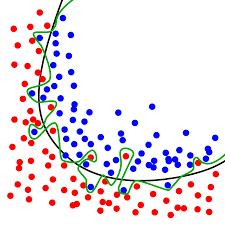
\includegraphics[width=0.4\textwidth]{Figs/section_4/overfitting.png}
		\caption{OverFitting in a neural network, \href{https://en.wikipedia.org/wiki/Overfitting}{Source}}
	\end{figure}
\end{frame}


\begin{frame}{Early Stopping}
	\begin{itemize}
		\item Stop the training procedure when the validation error is \tc{keywords}{minimum}.
	\end{itemize}
	\vspace{0.1\textheight}
	\begin{figure}
		\centering
		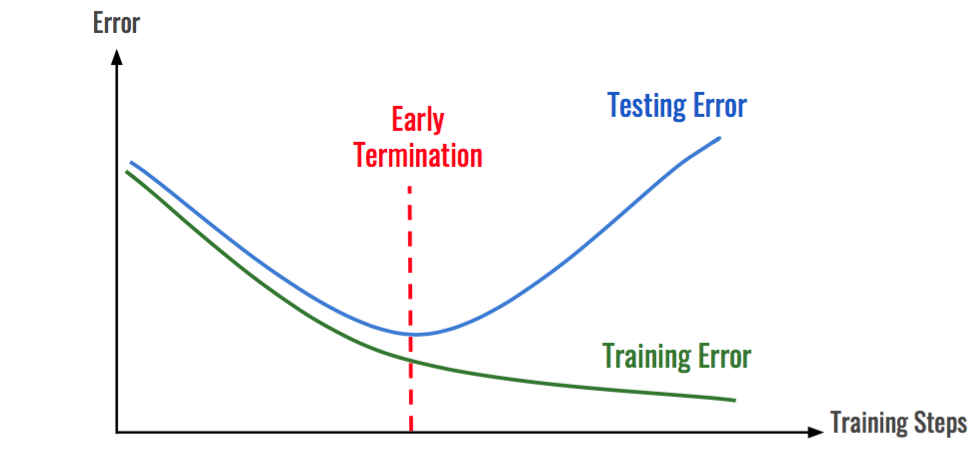
\includegraphics[width=0.8\textwidth]{Figs/Early Stopping.png}
		\caption{Early Stopping diagram, \href{https://medium.com/analytics-v7idhya/early-stopping-with-pytorch-to-restrain-your-model-from-overfitting-dce6de4081c5}{Source}}
	\end{figure}
\end{frame}

\begin{frame}{Dropout: Training Time}
	\begin{itemize}
		\item In each forward pass, \tc{keywords}{randomly} set some neurons to zero.
		\medskip
		\item The probability of dropping out for each neuron, which is called \tc{keywords}{dropout rate}, is a hyperparameter.
		\begin{itemize}
			\item 0.5 is a common dropout rate.
		\end{itemize}
		\medskip
		\item The probability of not dropping out is also called the \tc{keywords}{keep probability}.
	\end{itemize}
	\begin{figure}[H]
		\centering
		\begin{subfigure}[b]{0.45\textwidth}
			\centering
			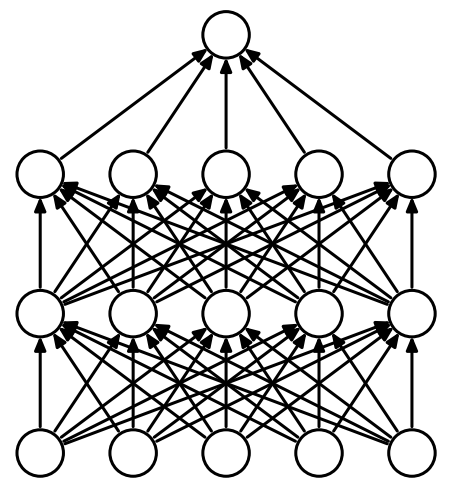
\includegraphics[height=0.4\textheight]{Figs/Dropout-before.png}
		\end{subfigure}
		\begin{subfigure}[b]{0.45\textwidth}
			\centering
			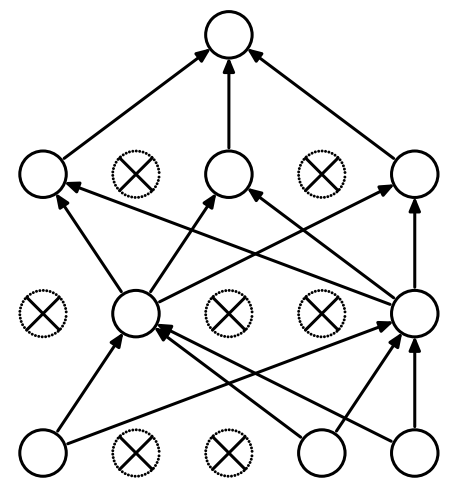
\includegraphics[height=0.4\textheight]{Figs/Dropout-after.png}
		\end{subfigure}
		\caption{Behavior of dropout at training time, \href{https://www.cs.toronto.edu/~hinton/absps/JMLRdropout.pdf}{Source}}
	\end{figure}
\end{frame}

%%%%%%%%%%%%%%%%%%%%%%%%%%%%%%%%%%%%%%[CNN]%%%%%%%%%%%%%%%%%%%%%%%%%%%%%%%%%%%%%%%%%%%%%%%%%%
\section{CNN}
\frame{\frametitle{Brief History of Computer Vision}
\begin{itemize}
    \item \Large{Before Deep Learning:} \large{\tc{keywords}{Hand-Crafted Features}}
\end{itemize}

\begin{figure}
    \centering
    \vspace{-0.3cm}

    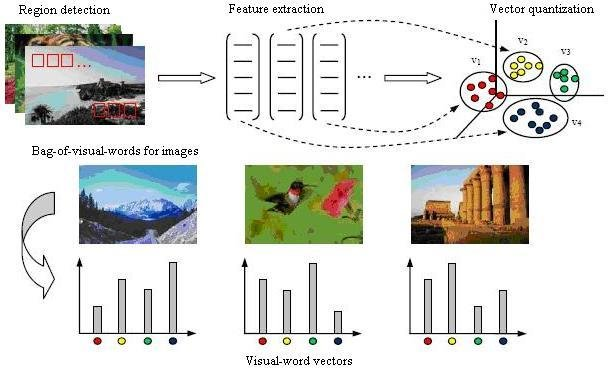
\includegraphics[width=0.8\columnwidth]{images/intro4.jpg} \caption{\cite{featureextrac2013}}
\end{figure}
}

\frame{\frametitle{CNNs}

\begin{itemize}
    \item \Large{What we've been using:}
    \begin{itemize}
        \item \large{Fully Connected Layers}
    \end{itemize}
\end{itemize}
\begin{figure}
    \centering
    \vspace{-0.2cm}
    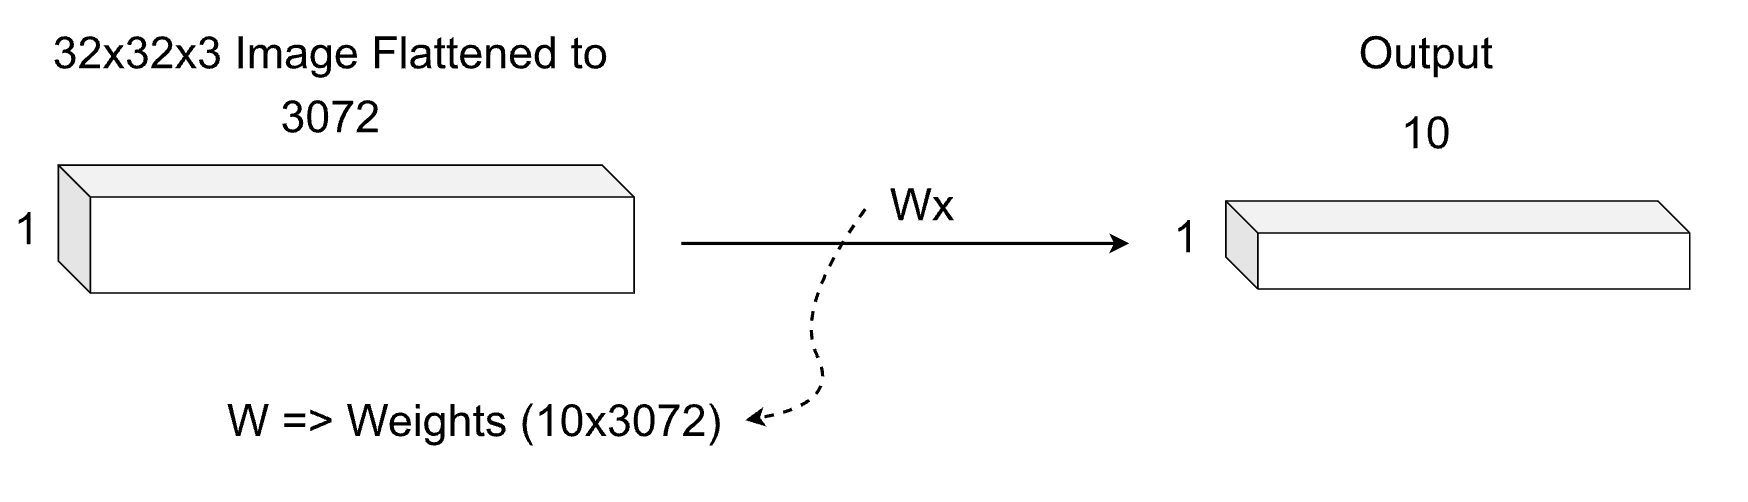
\includegraphics[width=1\columnwidth]{images/nnn}
\end{figure}
}

\frame{\frametitle{CNNs}
\begin{itemize}
    \item \Large{What we're going to learn:}
    \begin{itemize}
        \item \large{Convolutional Layer}
    \end{itemize}
\end{itemize}

\begin{figure}
    \centering
    \vspace{-0.3cm}

    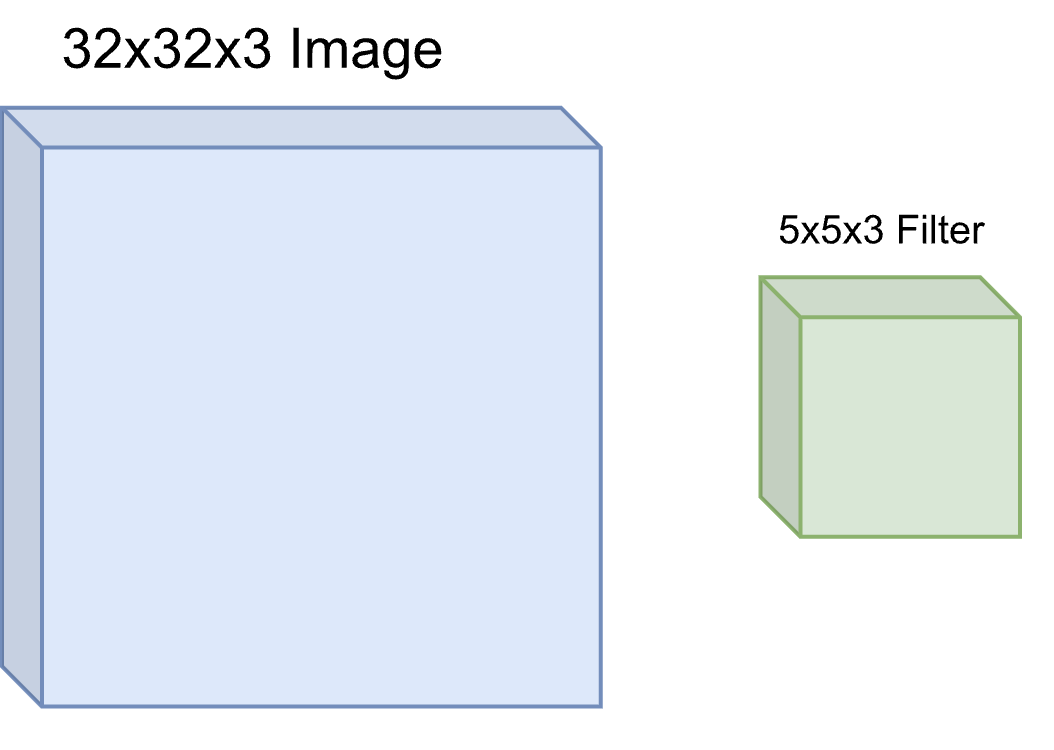
\includegraphics[width=0.6\columnwidth]{images/CNNN}
\end{figure}
}

\frame{\frametitle{What is Convolution and how does it work?}
    \begin{itemize}
        \item \normalsize This is how we calculate the convolutional layer's output:
    \end{itemize}
    \small
    \begin{equation*}
        Convolved Feature(i, j) = (I * K)(i, j) = \sum_{a=0}^{k_h - 1}\sum_{b=0}^{k_w - 1} I(i+a, j+b) K(a, b)
    \end{equation*}
        I: Input Image\newline
        K: Our Kernel\newline
        $k_h$ and $k_w$: The height and width of the Kernel

    \begin{figure}
    \centering
    \begin{minipage}{.1\textwidth}
      \centering
        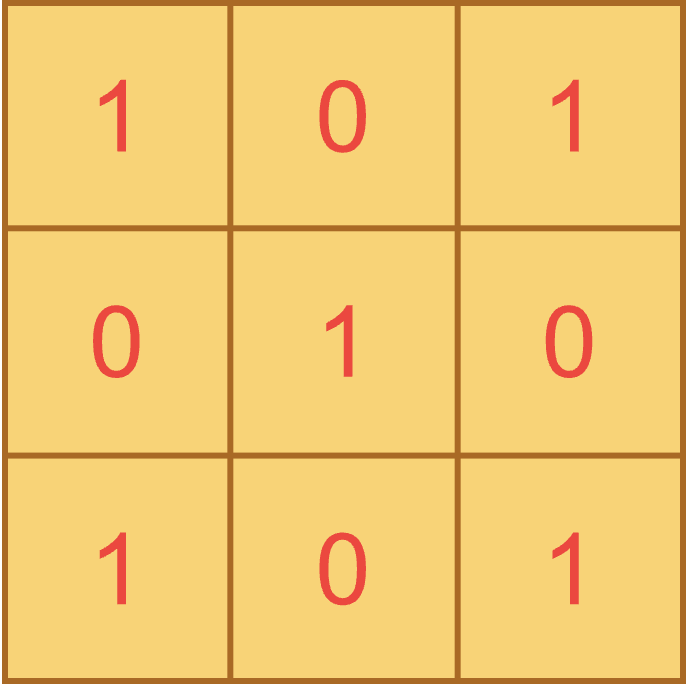
\includegraphics[width=0.7\columnwidth]{images/kernell}
        \caption{Convolving Kernel}
    \end{minipage}%
    \begin{minipage}{.9\textwidth}
      \centering
        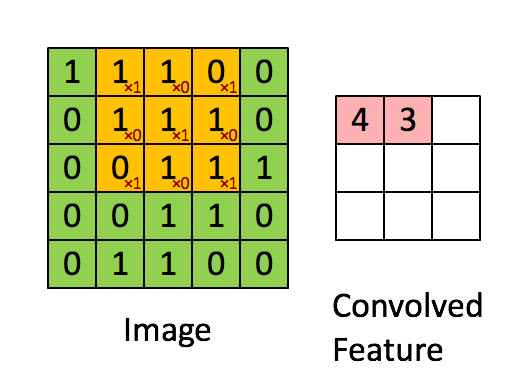
\includegraphics[width=0.45\columnwidth]{images/kernel-frame-1.png}
        \caption{Convoluting a 5x5x1 image with a 3x3x1 kernel to get a 3x3x1 convolved feature, \href{https://towardsdatascience.com/a-comprehensive-guide-to-convolutional-neural-networks-the-eli5-way-3bd2b1164a53}{Source}}
    \end{minipage}
	\end{figure}
}

\section{Implementation}
\frame{\frametitle{Implementation}
\begin{figure}
    \centering
    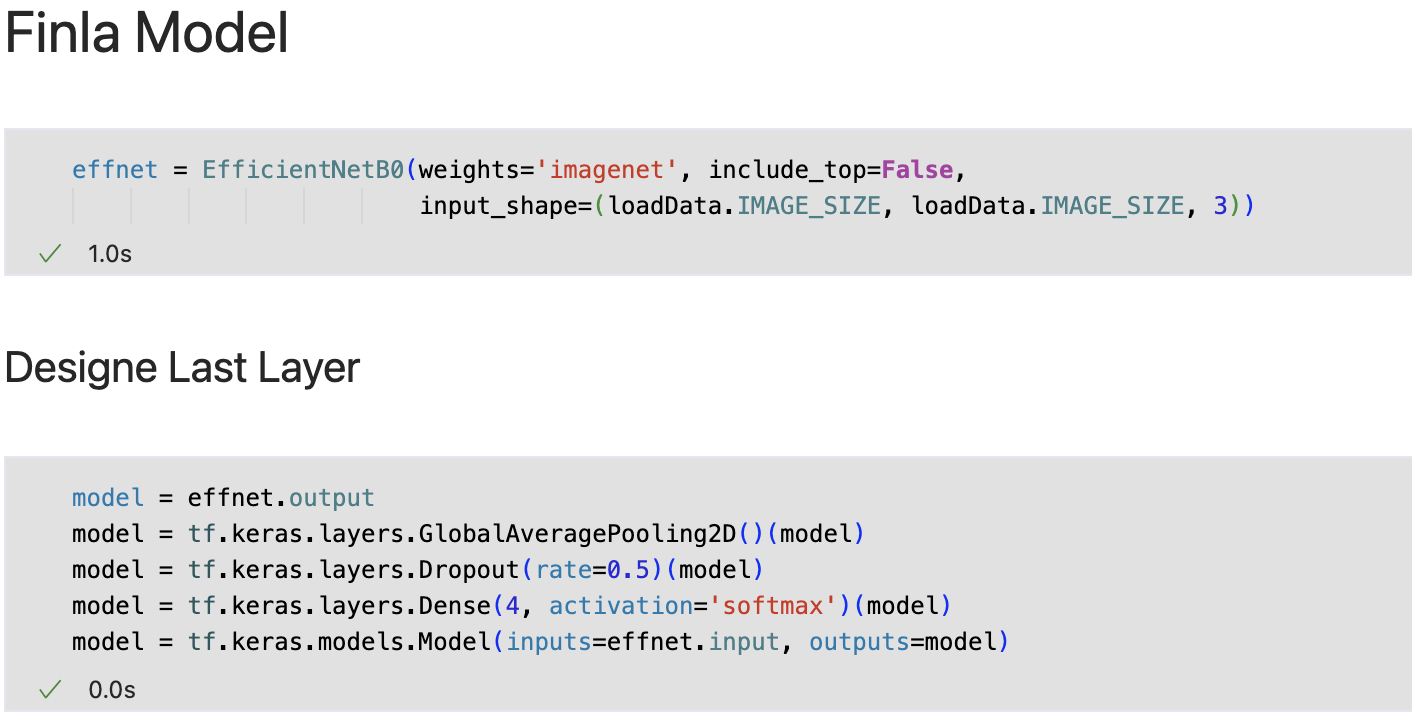
\includegraphics[width=0.9\columnwidth]{Figs/Model-im2}
\end{figure}
}

\section{Results}
\frame{\frametitle{Training}
\begin{figure}
    	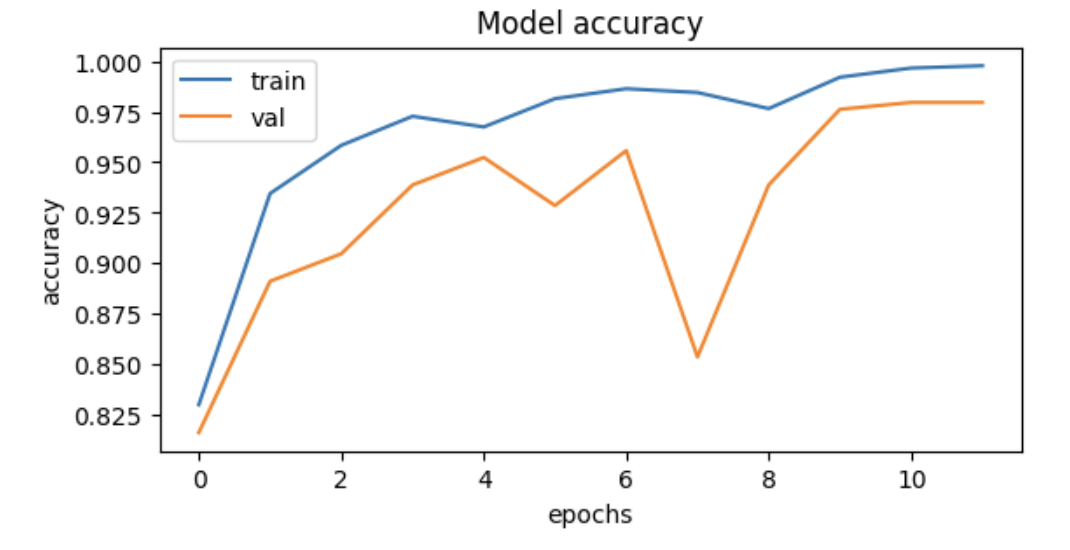
\includegraphics[width=0.6\columnwidth]{Figs/Model-acc}
    	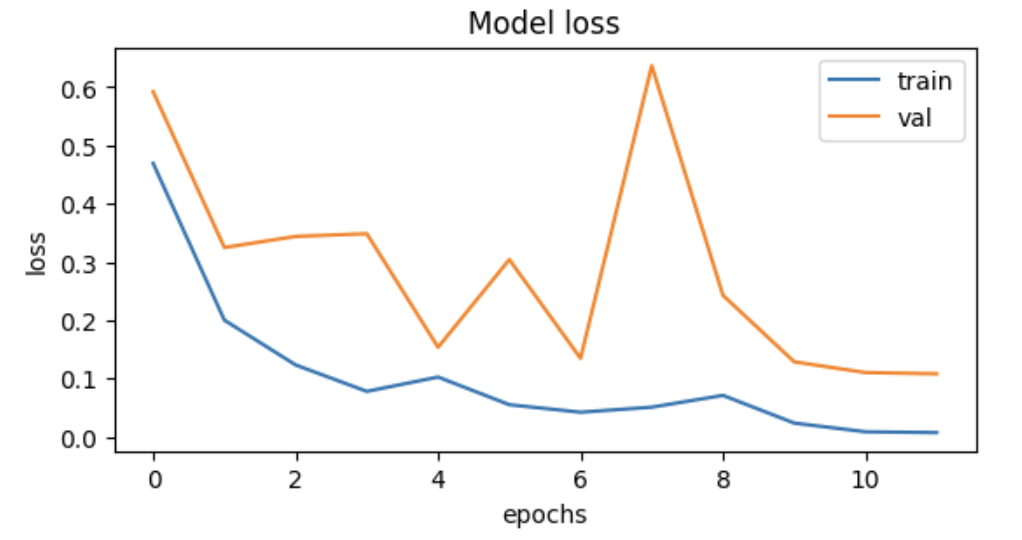
\includegraphics[width=0.6\columnwidth]{Figs/Model-loss}
\end{figure}
}


\frame{\frametitle{Confusion Matrix}
\begin{figure}
    	\includegraphics[width=0.8\columnwidth]{Figs/output.png}
\end{figure}
}


\frame{\frametitle{Accuracy $ \approx 97 \% !$}
\begin{figure}
    	\includegraphics[width=0.8\columnwidth]{Figs/acc}
\end{figure}
}
%%%%%%%%%%%%%%%%%%%%%%%%%%%%%%%%%%%%%%%%%%%%%%%%%%%%%%%%%%%%%%%%%%%%%%%%%%%%%%%%%%%%%%%%%%%%%%%
\section{}

\frame{
\centering
\vspace{60 pt}
\textbf{\Huge Thank You!}

\vspace{50pt}
\textbf{\Large Any Question?}
}

\frame{\frametitle{Refrences}
\begin{itemize}

	\item Introduction To Machine Learning, Dr. SharifiZarChi \hyperlink{https://maktabkhooneh.org/}{Link}
    
    \item Deep Learning for Vision Systems - Mohamed Elgendy - 2020 - \hyperlink{https://www.oreilly.com/library/view/deep-learning-for/9781617296192/}{Link}

		\item CS231n: Convolutional Neural Networks for Visual Recognition \hyperlink{https://cs231n.github.io/}{Link}
	
	\item Brain tumor intro - Mayo Clinic \hyperlink{https://www.mayoclinic.org/diseases-conditions/brain-tumor/symptoms-causes/syc-20350084}{Link}
\end{itemize}
}
%%%%%%%%%%%%%%%%%%%%%%%%%%%%%%%%%%%%%%%%%%
\end{document}